% A template for Wiley article submissions developed by 
% Overleaf for the Overleaf-Wiley pilot which ran 
% during 2017 and 2018.
% 
% This template is no longer supported, but is provided
% for historical reference. Last updated January 2019.
%
% Please note that whilst this template provides a 
% preview of the typeset manuscript for submission, it 
% will not necessarily be the final publication layout.
%
% Document class options:
% =======================
% blind: Anonymise all author, affiliation, correspondence
%        and funding information.
%
% lineno: Adds line numbers.
%
% serif: Sets the body font to be serif. 
%
% twocolumn: Sets the body text in two-column layout. 
% 
% num-refs: Uses numerical citation and references style 
%           (Vancouver-authoryear).
%
% alpha-refs: Uses author-year citation and references style
%             (rss).
%
% Using other bibliography styles:
% =======================
%
% To specify a different bibiography style
%
% 1) Do not use either num-refs or alpha-refs in documentclass.
% 2) Load natbib package with the options set as needed.
% 3) Use the \bibliographystyle command to specify the style
% 
% Included NJD styles are: 
%   WileyNJD-ACS
%   WileyNJD-AMA
%   WileyNJD-AMS
%   WileyNJD-APA
%   WileyNJD-Harvard
%   WileyNJD-VANCOUVER
%
% or you may upload an alternative .bst file 
% (if requested by the journal).
%
% Examples:
% =======================
%% Example: Using numerical, sort-by-authors citations.
\documentclass[num-refs]{wiley-article}
%\documentclass{wiley-article}
%\usepackage{lmodern}
\usepackage{amsmath, amssymb}
\usepackage{ragged2e}
%\usepackage{mathptmx}
%\usepackage{newtxmath}
%\usepackage{newtxtext,newtxmath}
\usepackage{braket}
\usepackage[T1]{fontenc}
\usepackage{hyperref}
\usepackage{graphicx}
\usepackage{upgreek}
\usepackage{textcomp}
\usepackage{booktabs}
\usepackage[utf8]{inputenc}
%\usepackage{newunicodechar}
\usepackage{xspace}
\usepackage{siunitx}
\sloppy

% --- Restore summation/integral symbols in Wiley class ---
%\makeatletter
%\DeclareSymbolFont{operators}{OT1}{cmr}{m}{n}
%\SetSymbolFont{operators}{bold}{OT1}{cmr}{bx}{n}
%\makeatother


%\usepackage[nothead]{makecell}
%% Example: Using author-year citations and anonymising submission
% \documentclass[blind,alpha-refs]{wiley-article}

%% Example: Using unsrtnat for numerical, in-sequence citations
% \documentclass{wiley-article}
% \usepackage[numbers]{natbib}
% \bibliographystyle{unsrtnat}

%% Example: Using WileyNJD-AMA reference style and superscript
%%          citations, two-column and serif fonts for AIChE
% \documentclass[serif,twocolumn,lineno]{wiley-article}
% \usepackage[super]{natbib}
% \bibliographystyle{WileyNJD-AMA}
% \makeatletter
% \renewcommand{\@biblabel}[1]{#1.}
% \makeatother

% Add additional packages here if required

% Update article type if known
\papertype{Original Article}
% Include section in journal if known, otherwise delete
\paperfield{Journal Section}

%\title{Quantum Simulations of Battery Electrolytes with VQE–qEOM and SQD: Active-Space Design, Dissociation, and Excited States of LiPF$_6$, NaPF$_6$, and FSI Salts}

\title{Quantum Simulations of Battery Electrolytes Using Variational Quantum 
Eigensolver, Equation-of-Motion, and Sample-Based Diagonalization Methods: 
Active-Space Design, Dissociation, and Excited States of LiPF$_6$, NaPF$_6$, and FSI Salts}

% List abbreviations here, if any. Please note that it is preferred that abbreviations be defined at the first instance they appear in the text, rather than creating an abbreviations list.
%\abbrevs{ABC, a black cat; DEF, doesn't ever fret; GHI, goes home immediately.}

% Include full author names and degrees, when required by the journal.
% Use the \authfn to add symbols for additional footnotes and present addresses, if any. Usually start with 1 for notes about author contributions; then continuing with 2 etc if any author has a different present address.
\author[1]{Sk Mujaffar Hossain}
\author[1,2\authfn{1}]{Seung-Cheol Lee}
\author[1\authfn{1}]{Satadeep Bhattacharjee}

%\contrib[\authfn{1}]{Equally contributing authors.}

% Include full affiliation details for all authors
\affil[1]{Indo-Korea Science and Technology Center (IKST), Bengaluru 560064, India}
\affil[2]{Electronic Materials Research Center, Korea Institute of Science and Technology (KIST), Seoul 02792, Republic of Korea}


\corraddress{Indo-Korea Science and Technology Center (IKST), Bengaluru 560064, India}

%\corremail{leesc@kist.re.kr}
%\corremail{gour.das@tcgcrest.org}
\corremail{leesc@kist.re.kr, s.bhattacharjee@ikst.res.in}

%\presentadd[\authfn{1}]{Indo-Korea Science and Technology Center (IKST), Bengaluru 560064, India}

\fundinginfo{This work was supported by the Korea Institute of Science and Technology (Grant number 2E31851)}

% Include the name of the author that should appear in the running header
\runningauthor{SK. M. Hossain et al.}

\begin{document}

\begin{frontmatter}
\maketitle

\begin{abstract}
Accurate prediction of excited states in battery electrolytes is crucial for understanding photostability, oxidative stability, and degradation. We employ hybrid quantum–classical algorithms—the Variational Quantum Eigensolver (VQE) for ground states and the quantum equation of motion (qEOM) for vertical singlet excitations to study LiPF$_6$, NaPF$_6$, LiFSI, and NaFSI. Compact active spaces from frontier orbitals were mapped to qubits and reduced via symmetry tapering and commuting-group measurements to lower sampling cost. Within $\sim$10-qubit models, VQE-qEOM agrees closely with exact diagonalization, while sample-based quantum diagonalization (SQD) in larger spaces recovers near-exact (subspace-FCI) energies. Spectra show clear anion–cation trends within the VQE–qEOM framework: PF$_6$ salts have higher first-excitation energies (LiPF$_6$~$\approx$13.2~eV) and a compact three-state cluster at 12–13~eV, whereas FSI salts exhibit lower onsets ($\approx$8–9~eV) with nearly degenerate S$_1$ and S$_2$ states and a higher S$_3$ separated by $\sim$1.3~eV.
Independent TDDFT calculations yield systematically lower absolute excitation energies but reproduce the same anion- and cation-dependent trends, confirming that the relative ordering and physical interpretation of the quantum results are robust. Replacing Li$^+$ with Na$^+$ narrows the gap by $\sim$0.4–0.8 eV per anion family. Converting S$_1$ to wavelengths places onsets in the deep UV (LiPF$_6$ 94 nm; NaPF$_6$ 100 nm; LiFSI 141 nm; NaFSI 148 nm). Results for isolated species or embedded clusters are NISQ-feasible, with solvent shifts incorporable via classical $\Delta$-solvation. Current quantum algorithms capture excitation trends, advancing electrolyte design.

%\begin{abstract}
%Accurate prediction of electronically excited states in battery electrolytes is essential for understanding photostability, oxidative stability, and degradation pathways. Here, we employ hybrid quantum--classical algorithms—the Variational Quantum Eigensolver (VQE) for ground states and the quantum equation-of-motion (qEOM) formalism for vertical singlet excitations—to study LiPF$_6$, NaPF$_6$, LiFSI, and NaFSI salts. Compact active spaces constructed from frontier orbitals are mapped to qubits and reduced via symmetry tapering and commuting-group measurements to minimize sampling cost. Within $\sim$10-qubit models, VQE–qEOM reproduces exact diagonalization results within the same active spaces, while sample-based quantum diagonalization (SQD) in enlarged spaces recovers near-exact (subspace-FCI) ground-state energies.

%The excitation spectra reveal clear anion- and cation-dependent trends: PF$_6$ salts exhibit higher first-excitation energies (LiPF$_6$ $\approx$ 13.2 eV) and a compact three-state manifold near 12--13 eV, whereas FSI salts show lower onsets ($\approx$ 8--9 eV) with nearly degenerate S$_1$ and S$_2$ states and a higher S$_3$ separated by $\sim$1.3 eV. Independent TDDFT calculations systematically lower absolute excitation energies but reproduce the same relative ordering across anion and cation families, supporting the robustness of the quantum-derived trends. Substituting Li$^+$ with Na$^+$ consistently narrows the excitation gap by $\sim$0.4--0.8 eV. Mapping the lowest excitations to wavelengths places all absorption onsets in the deep-ultraviolet regime. These results demonstrate that current NISQ-era quantum algorithms can capture chemically meaningful excitation trends in electrolyte salts, providing a viable foundation for quantum-assisted electrolyte design.


% Please include a maximum of seven keywords
\keywords{\emph{Quantum Computing}, \emph{VQE}, \emph{qEOM}, \emph{SQD}, \emph{Li and Na electrolyte Salt}, \emph{Active Space}, \emph{Excited States}, \emph{photostability}}

\end{abstract}

\end{frontmatter}

%%%%%%%%%%%%%%%%%%%%%%%%%%%%%%%%%%%%%%%%%%%%%%%%%%%%%%%%%%%%%%%%%%%%%
%% Start the main part of the manuscript here.
%%%%%%%%%%%%%%%%%%%%%%%%%%%%%%%%%%%%%%%%%%%%%%%%%%%%%%%%%%%%%%%%%%%%%
\section{Introduction}

The rapid development of electrochemical energy storage technologies has created an urgent demand for stable, high-performance electrolytes. In lithium-ion batteries (LIBs), and increasingly in sodium-ion batteries (SIBs), electrolyte salts such as LiPF$_6$, NaPF$_6$, LiFSI, and NaFSI \cite{he2025research} play a pivotal role in determining ionic conductivity, oxidative stability, and long-term durability. However, the excited-state properties of these salts remain poorly understood, despite their direct relevance to photostability, oxidative degradation, and safety under extreme conditions. Classical approaches such as density functional theory (DFT) and post-Hartree--Fock methods have provided valuable insights, yet they face well-known limitations in treating electron correlation and excited states in complex molecular systems. 

%Recent advances in quantum computing offer a promising alternative\cite{patel2025quantum}, hybrid quantum--classical algorithms such as the Variational Quantum Eigensolver (VQE)\cite{peruzzo2014variational,boyn2021quantum} and its extension with the quantum Equation-of-Motion (qEOM)\cite{zheng2024quantum,hlatshwayo2024quantum} provide a scalable framework for accessing both ground and excited states on noisy intermediate-scale quantum (NISQ) devices \cite{bharti2022noisy,acampora2023d,de2023complete}. In this work, we leverage VQE, qEOM, and sample-based quantum diagonalization (SQD)\cite{robledo2025chemistry,yu2025quantum,kanno2023quantum,sugisaki2024hamiltonian} to investigate representative battery electrolytes, establishing chemically accurate benchmarks and revealing systematic trends in stability across PF$_6$- and FSI-based salts as well as Li$^+$/Na$^+$ analogues.

Recent advances in quantum computing provide a promising route for simulating many-body electronic structure by enabling direct representation of molecular Hamiltonians on qubit-based devices\cite{patel2025quantum,cao2019quantum}. Within this framework, hybrid quantum--classical algorithms such as the Variational Quantum Eigensolver (VQE)\cite{peruzzo2014variational,boyn2021quantum,mcclean2016theory} and its extension through the quantum Equation-of-Motion (qEOM)\cite{zheng2024quantum,hlatshwayo2024quantum} offer scalable strategies for accessing ground- and excited-state energies in the noisy intermediate-scale quantum (NISQ) regime\cite{ollitrault2020quantum,de2023complete,bharti2022noisy,acampora2023d}. VQE has been successfully demonstrated for a range of small molecular systems, including H$_2$, LiH, BeH$_2$, H$_4$, HeH$^+$, and CO$_2$\cite{peruzzo2014variational,mcclean2016theory,o2016scalable,ghosh2023deep,tao2022exploring,lotstedt2022evaluation,bauer2020quantum}, and extended to larger molecules through symmetry-based qubit reduction and tailored variational ans\"atze\cite{cao2019quantum}. Complementary to VQE--qEOM, sample-based quantum diagonalization (SQD)\cite{robledo2025chemistry,yu2025quantum,kanno2023quantum,sugisaki2024hamiltonian} provides a systematic pathway to recover near-exact eigenvalues in enlarged active spaces, thereby strengthening the benchmarking and scalability of quantum simulations. Together, these quantum algorithms have been applied across diverse areas of chemistry and materials science, including drug discovery, catalysis, organic photovoltaics, strongly correlated materials, and nonadiabatic molecular dynamics\cite{bauer2020quantum,blunt2022perspective,cava2021introduction,delgado2025quantum,hariharan2024modeling,lipka2024catalysis,motta2020quantum,ollitrault2020nonadiabatic,miessen2021quantum}. These advances highlight the growing maturity and versatility of quantum approaches, motivating their application to chemically complex and technologically relevant systems such as battery electrolyte salts, where accurate excited-state descriptions remain challenging for classical methods.


%Recent advances in quantum computing provide a promising alternative by enabling direct simulation of many-body electronic structures on qubit-based devices\cite{patel2025quantum,cao2019quantum}. Hybrid quantum--classical algorithms such as the Variational Quantum Eigensolver (VQE)\cite{peruzzo2014variational,boyn2021quantum, mcclean2016theory} and its extension with the quantum Equation-of-Motion (qEOM)\cite{zheng2024quantum,hlatshwayo2024quantum} offer scalable strategies for accessing both ground- and excited-state energies within the noisy intermediate-scale quantum (NISQ) regime \cite{peruzzo2014variational,mcclean2016theory,ollitrault2020quantum,de2023complete,bharti2022noisy,acampora2023d}. Complementary to VQE--qEOM, sample-based quantum diagonalization (SQD)\cite{robledo2025chemistry,yu2025quantum,kanno2023quantum,sugisaki2024hamiltonian} provides a systematic route to recover nearly exact eigenvalues in larger active spaces, thereby extending the accuracy and benchmarking capability of quantum simulations. Together, these methods open new possibilities for probing photo-induced processes, excitation spectra, and stability trends in battery electrolytes beyond the reach of classical approaches.

%Recent efforts have applied quantum algorithms to chemical and materials problems, demonstrating their potential but also highlighting key challenges\cite{patel2025quantum,sureshbabu2021implementation}. The VQE has been successfully employed for small molecules as toy model such as H$_2$, LiH, BeH$_2$, H$_4$, HeH$^+$, and CO$_2$\cite{peruzzo2014variational,mcclean2016theory,o2016scalable,ghosh2023deep, tao2022exploring,lotstedt2022evaluation,bauer2020quantum}, and extended to larger systems using symmetry-based qubit reduction and tailored ans\"atze \cite{cao2019quantum}. Beyond all these studies, quantum computations are increasingly being explored in diverse fields such as drug discovery \cite{cao2019quantum,bauer2020quantum, blunt2022perspective,cava2021introduction,delgado2025quantum}, sustainable catalysis \cite{hariharan2024modeling,lipka2024catalysis,von2021quantum}, organic photovoltaics \cite{ollitrault2020quantum}, strongly correlated quantum materials \cite{motta2020quantum}, electronic structure\cite{barkoutsos2018quantum}, and nonadiabatic molecular quantum dynamics\cite{ollitrault2020nonadiabatic,miessen2021quantum}. These applications demonstrate the broad potential of quantum algorithms to address problems across chemistry, materials science, and biology, further motivating their deployment in complex molecular systems such as battery electrolytes. These advances highlight the versatility of quantum approaches across diverse domains of chemistry, from biomolecular design to energy materials\cite{paudel2022quantum}.The qEOM approach has further enabled access to electronically excited states, providing chemically accurate excitation energies in benchmark systems \cite{ollitrault2020quantum,mcardle2020quantum}. 

More recently, applications have begun to emerge in energy materials\cite{paudel2022quantum}, including quantum simulations of sulfur species in lithium--sulfur batteries \cite{rice2021quantum}, organic emitters \cite{gao2021applications}, and transition-metal complexes \cite{ghosh2023deep}. Despite these advances, systematic studies of realistic electrolyte salts, particularly those relevant for Li- and Na-ion batteries, remain unexplored. In this context, our work establishes a framework that integrates VQE, qEOM, and SQD to capture both ground- and excited-state properties of complex electrolyte systems with chemical accuracy, while revealing chemically meaningful trends in photostability and oxidative stability.

Quantum algorithms for chemistry have significantly improved the feasibility of applying variational quantum eigensolvers (VQE) to chemically relevant systems. Progress in active-space selection, orbital embedding, and symmetry exploitation has enabled accurate treatment of molecular ground and excited states within compact qubit registers, even in the NISQ regime. Techniques such as adaptive active-space construction, frozen-core approximations, and embedded VQE frameworks have been shown to systematically recover correlation effects while controlling circuit depth and measurement cost \cite{alfonso2025chemical,lim2024fragment}. These developments provide a practical foundation for extending VQE-based approaches beyond toy molecules and motivate the active-space and qubit-reduction strategies adopted in the present work.

It is important to note that current quantum hardware operates in the noisy intermediate-scale quantum (NISQ) regime, where decoherence, gate imperfections, and readout errors limit circuit depth and measurement fidelity. As a result, many chemically relevant quantum simulations—including those based on the variational quantum eigensolver (VQE) and quantum equation-of-motion (qEOM)—are presently carried out on noiseless simulators to establish methodological accuracy and chemical validity. Addressing the impact of hardware noise through error mitigation strategies remains a central challenge for extending such approaches to real quantum devices.

The ion-pair models studied here are intended as controlled gas-phase reference systems for benchmarking quantum algorithms, rather than as explicit representations of bulk electrolyte speciation. In real electrolytes, ion pairing depends on concentration, solvent polarity, and temperature; however, excitation energies and stability trends are primarily governed by the intrinsic electronic structure of the anionic moieties. By combining ion-pair and isolated-anion benchmarks, this work isolates chemically meaningful trends while remaining compatible with near-term quantum hardware constraints.

In this work, we apply the Variational Quantum Eigensolver combined with the quantum equation-of-motion (VQE–qEOM) framework to investigate the ground and low-lying excited states of four representative electrolyte salts: LiPF$_6$, NaPF$_6$, LiFSI, and NaFSI. The study focuses on systematic active-space construction, qubit reduction strategies, and controlled benchmarking against classical electronic-structure methods, with sample-based quantum diagonalization (SQD) employed to assess scalability beyond compact quantum models. In addition to excitation energies, we examine HOMO–LUMO gaps and cation–anion dissociation profiles that are relevant to photoinduced processes in battery electrolytes. All quantum simulations are performed for isolated species or embedded cluster models compatible with current NISQ-era resources, providing a well-defined framework for evaluating quantum algorithms on chemically relevant electrolyte systems.


\section{Methodology}

\subsection{Workflow of Quantum Simulation}
In this study, we investigated the ground and excited state properties of representative electrolyte salts, including LiPF$_6$, NaPF$_6$, LiFSI, and NaFSI, using hybrid quantum--classical algorithms. The workflow in Figure \ref{fig:workflow} consisted of (i) construction of active spaces from \textit{ab initio} orbital energies, (ii) mapping of the molecular Hamiltonian to qubit operators, (iii) ground-state optimization using the Variational Quantum Eigensolver (VQE)\cite{bauer2020quantum}, (iv) excited-state calculations using the quantum Equation-of-Motion (qEOM) formalism, and (v) benchmarking and scaling analysis using Sample-based Quantum Diagonalization (SQD)\cite{robledo2025chemistry}. All quantum simulations were implemented using IBM Qiskit \cite{matthew_treinish_2023_8190968}, which was executed primarily on noiseless statevector simulators, with selected SQD benchmark runs performed on real quantum hardware.


\begin{figure}[htp]
    \centering
    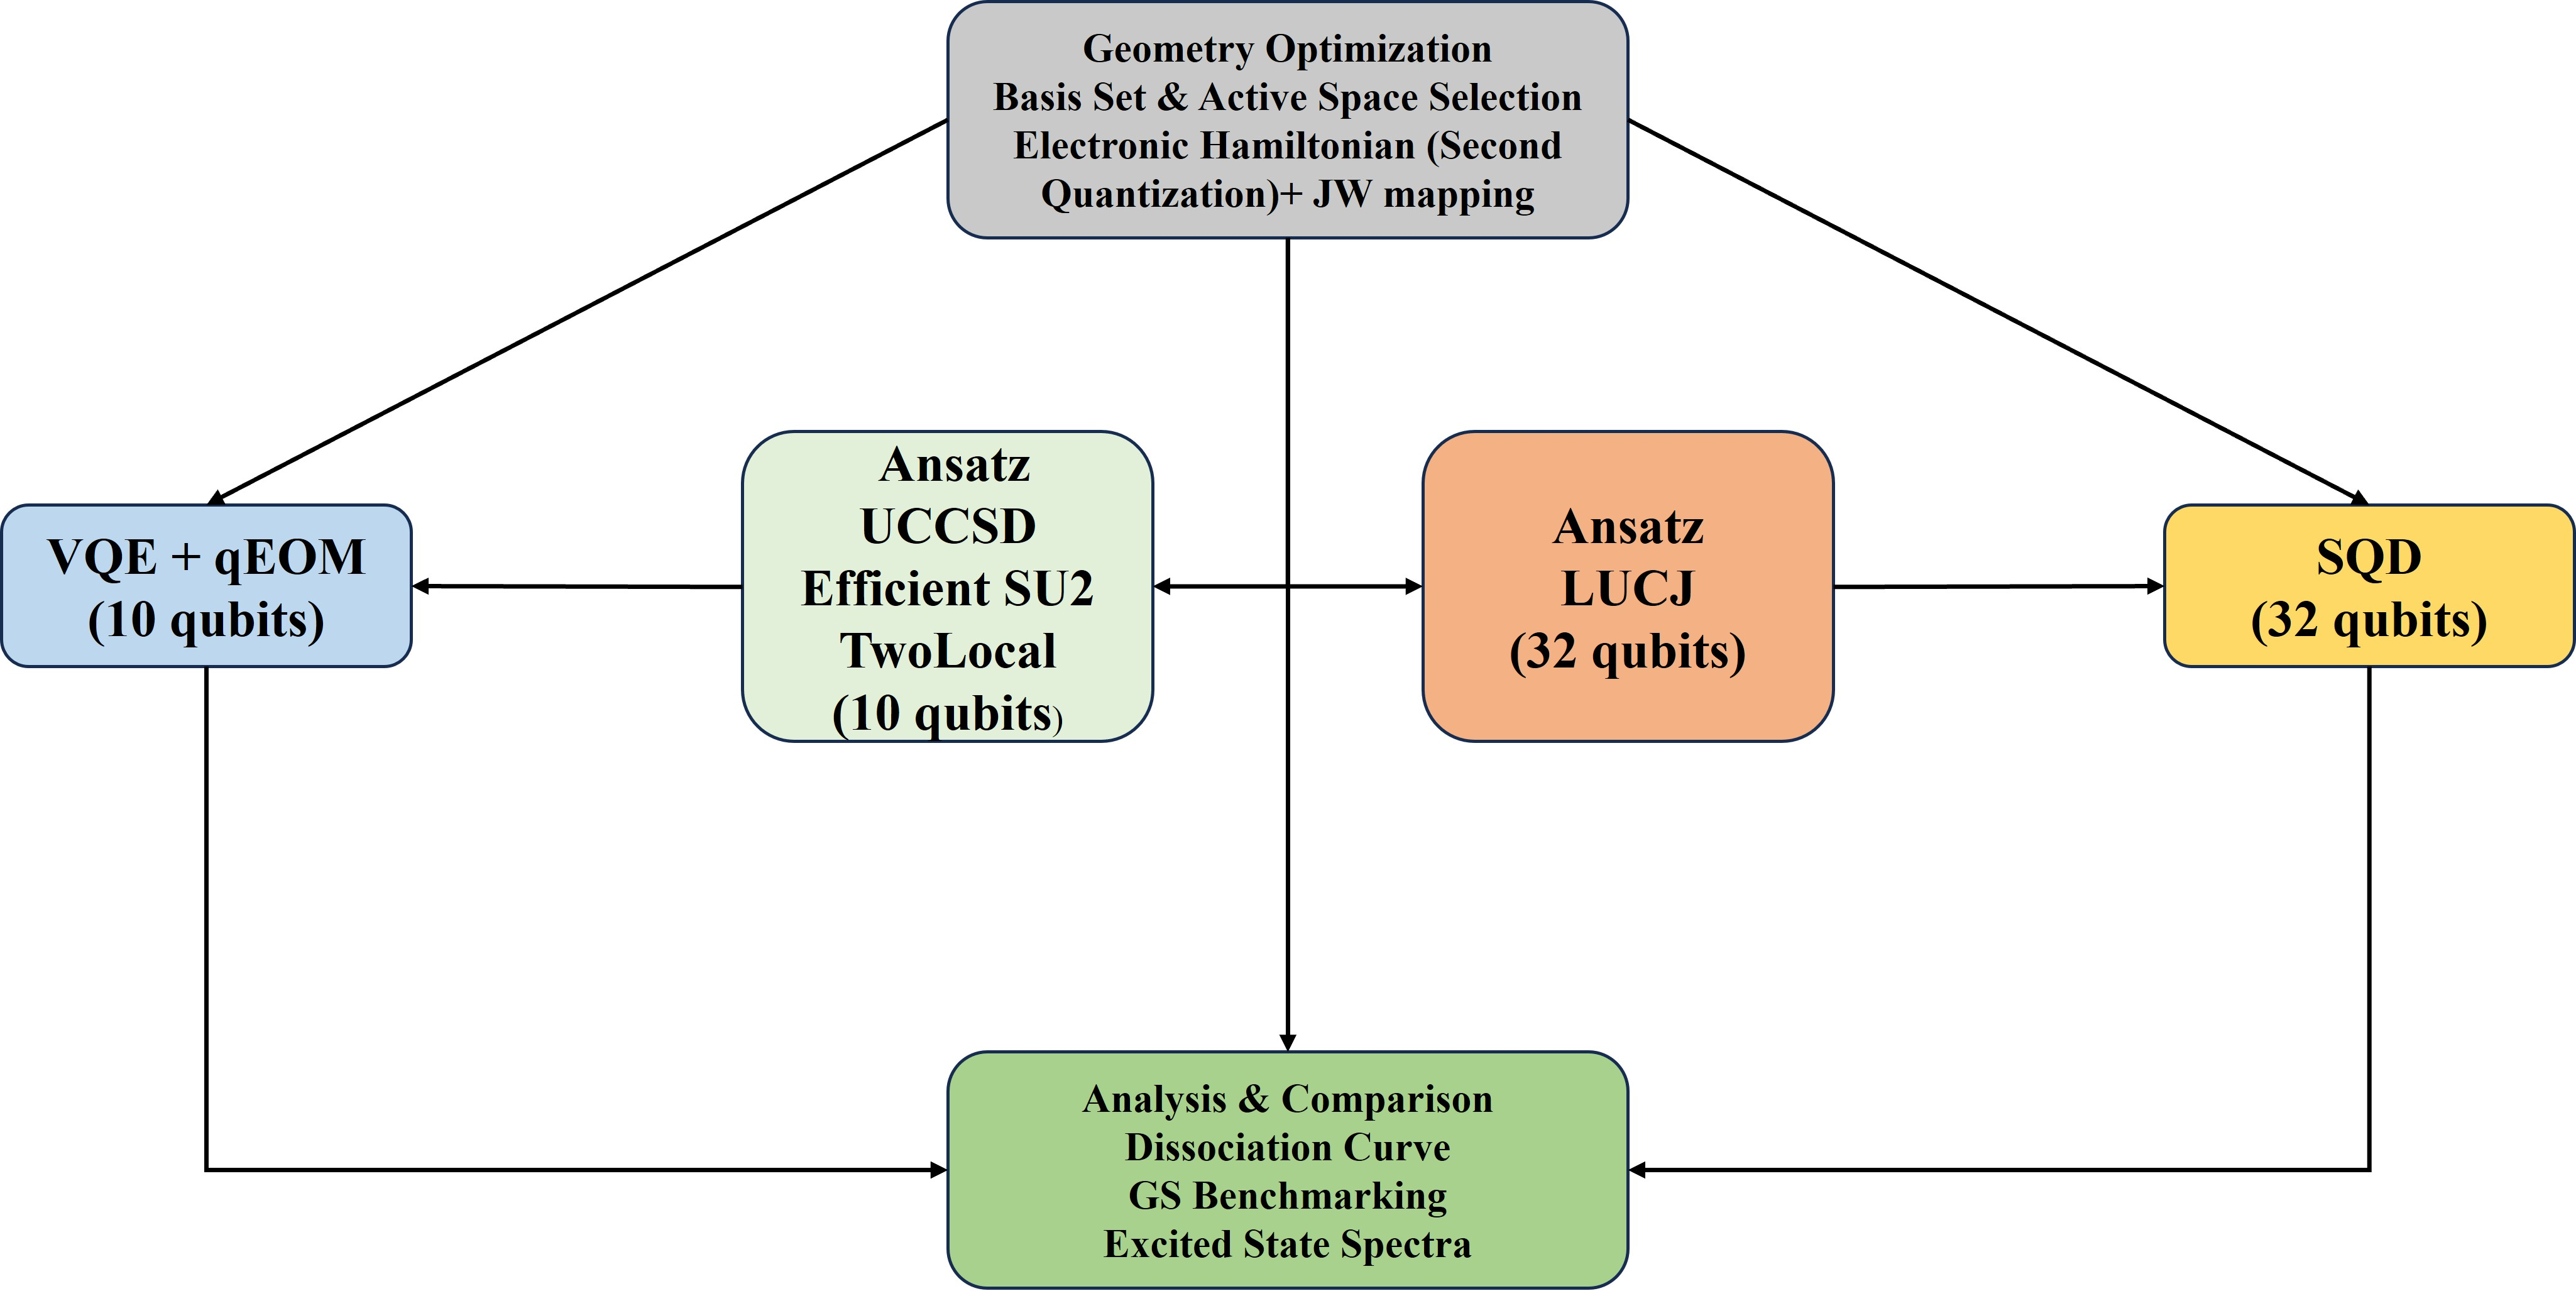
\includegraphics[width=12.5cm]{workflow_1.jpg}
    \caption{Workflow of quantum simulation study of molecular electrolytes.}
    \label{fig:workflow}
\end{figure}

\subsection{Geometry Optimization, Basis Set Choice, and Active Space Design}

The molecular geometries of LiPF$_6$, NaPF$_6$, LiFSI, and NaFSI were optimized at the B3LYP/6-311+G(d,p) level of theory using the Gaussian software package\cite{g16}. For quantum computations, several basis sets (STO-3G, 6-31G, cc-pVDZ and cc-pVTZ) were benchmarked to balance computational cost and accuracy. The cc-pVDZ basis set was ultimately selected for production runs, as it most widely used \cite{kaliakin2025implicit} and provides a reliable compromise between capturing electronic correlation and maintaining tractable quantum resource requirements.  

Active spaces were systematically constructed by freezing chemically inert core orbitals and retaining only the valence orbitals near the HOMO–LUMO frontier. This strategy reduced the number of required qubits from more than 200 in the full orbital space to a practical range of 4 to 12 qubits, while preserving the essential correlation effects required for chemical accuracy. The active-space choices were further validated by inspecting molecular orbital visualizations and natural occupation numbers, ensuring that the reduced spaces retained all electronically relevant contributions. This protocol follows best practices established in recent active space design studies for quantum simulations of the NISQ era \cite{motta2020quantum, tilly2022variational}.The same active-space construction protocol was later validated through isolated anion benchmark calculations, as discussed in Section~\ref{tab:anion_casci}.


\subsection{Electronic Hamiltonian and Qubit Mapping}

The molecular ground state was obtained through the Rayleigh--Ritz variational principle, which guarantees the following.

\begin{equation}
\langle \Psi(\vec{\Theta}) \,|\, \hat{H} \,|\, \Psi(\vec{\Theta}) \rangle \geq E_{0},
\end{equation}

where $\Psi(\vec{\Theta})$ is a parametrized trial wavefunction, $\hat{H}$ is the molecular Hamiltonian operator, and $E_{0}$ is the exact ground state energy. Within the VQE framework, the parameters $\vec{\Theta}$ are variationally optimized such that the expectation value approaches $E_{0}$ as closely as possible on quantum hardware or simulators.

The molecular electronic Hamiltonian $\hat{H}$ was expressed in second quantization within the Born--Oppenheimer approximation as\cite{de2023complete,ghosh2023deep,gao2021applications}

\begin{equation}
\hat{H} = \sum_{pq} h_{pq} \, a_p^\dagger a_q 
+ \tfrac{1}{2} \sum_{pqrs} h_{pqrs} \, a_p^\dagger a_q^\dagger a_r a_s
\end{equation}

where $a_p^\dagger$ and $a_q$ are fermionic creation and annihilation operators, $h_{pq}$ are one-electron integrals (kinetic energy and nuclear attraction), and $h_{pqrs}$ are two-electron repulsion integrals in an orthonormal molecular orbital basis and these one and two-electron integrals were obtained using the PySCF package.\cite{matthew_treinish_2023_8190968,sun2020recent,sun2018pyscf,ekström2010arbitrary}
For quantum simulation, the fermionic Hamiltonian was mapped to qubit operators using the Jordan--Wigner (JW)\cite{jordan1928pauli,ortiz2002simulating,somma2002simulating} transformation, which preserves the fermionic anticommutation relations by introducing non-local strings of Pauli operators. The resulting qubit Hamiltonian takes the generic form
\begin{equation}
\hat{H} = \sum_i c_i P_i = \sum_i c_i\prod_j\sigma_j^i 
\end{equation}
where $c_i$ are real coefficients derived from molecular integrals and $P_i$ are tensor products of Pauli operators $\sigma$ ($I$, $X$, $Y$, $Z$)\cite{de2023complete}. This qubit representation serves as the input for the VQE and subsequent qEOM excited-state calculations.

\subsection{Variational Quantum Eigensolver (VQE)}
The VQE algorithm was used to obtain ground-state wavefunctions by variationally minimizing the expectation value of the molecular Hamiltonian on a quantum device or simulator.\cite{peruzzo2014variational,mcclean2016theory,grimsley2019adaptive} 
Fermionic Hamiltonians were mapped to qubit operators via the Jordan--Wigner transformation, and several ans\"atze were benchmarked, including hardware-efficient forms (EfficientSU2, TwoLocal) and the chemically motivated UCCSD.\cite{peruzzo2014variational,romero2018strategies,grimsley2019trotterized,evangelista2019exact,kandala2017hardware} 
Although UCCSD entails greater circuit depth and is less NISQ-friendly, it consistently delivered the highest accuracy for electron correlation, in line with prior studies.\cite{innan2024quantum}

Classical optimization employed gradient-free COBYLA\cite{powell1994direct} (maximum 1000 iterations). 
Convergence was monitored using both the energy change (threshold $\Delta E \le 10^{-9}$~Ha) and the energy variance. 
The optimized ground state $|\psi_0\rangle$ served as the reference for all qEOM excited-state calculations. To reduce measurement cost, Pauli terms were grouped by qubit-wise commutativity. 
Unless otherwise noted, typical budgets were $5{\times}10^3$--$2{\times}10^4$ shots per geometry point under the same $\Delta E \le 10^{-9}$~Ha convergence criterion.


\subsection{Quantum Equation-of-Motion (qEOM)}

To investigate electronically excited states, we employed the quantum equation-of-motion (qEOM) formalism, which builds upon the VQE-optimized ground state reference by invoking a linear response framework \cite{ollitrault2020quantum,santagati2018witnessing,higgott2019variational,mcclean2017hybrid,colless2018computation}. In this method, excitation operators $\hat{R}_i$ are constructed within the particle-conserving subspace, typically including single and double excitations relative to the ground state. The excited-state ansatz takes the form
\begin{equation}
|\psi_i\rangle = \hat{R}_i |\psi_0\rangle ,
\end{equation}
where $|\psi_0\rangle$ is the VQE ground state and $\hat{R}_i$ acts as an excitation operator.  

The excitation energies $\omega_i$ are obtained by solving the eigenvalue equation
\begin{equation}
[\hat{H}, \hat{R}_i] |\psi_0\rangle = \omega_i \hat{R}_i |\psi_0\rangle ,
\end{equation}
which, in practice, is recast into a generalized eigenvalue problem by evaluating the commutator matrix elements on a quantum device or simulator. This procedure yields the low-lying vertical excitation spectrum directly from the ground-state reference, without the need for separate state-specific variational optimizations.  

The qEOM approach has been demonstrated to provide chemically accurate excitation energies for small and medium-sized molecules \cite{mcardle2020quantum,fan2021equation}, and is particularly attractive in the NISQ era because it leverages the compact ground-state wavefunction from VQE while accessing a manifold of excited states at comparable cost. In the context of battery electrolytes, qEOM enables characterization of photo-induced excitations and charge-transfer processes that are crucial for understanding stability and degradation mechanisms under operating conditions.


%\subsection{Sample-based Quantum Diagonalization (SQD)}
%While VQE + qEOM provided chemically accurate results within reduced active spaces (10 qubits), we further employed Sample-based Quantum Diagonalization (SQD) to benchmark accuracy in larger orbital subspaces. SQD is a projector-based algorithm that estimates matrix elements of the Hamiltonian via stochastic quantum sampling and then diagonalizes the effective Hamiltonian classically \cite{huggins2022unbiasing,lee2022unbiasing}. This allows recovery of near-exact eigenvalues with larger qubit counts (up to 32 in this work) at polynomial sampling cost. Recent work has demonstrated that SQD can achieve systematic improvements in accuracy and serve as a scalable benchmark for correlated electronic systems \cite{kaliakin2025implicit}. In this study, SQD therefore served both as a reference for validating compact VQE calculations and as a means of systematically recovering correlation energy in larger active spaces.

%\subsection{Sample-Based Quantum Diagonalization (SQD)}

%While VQE combined with qEOM provided chemically accurate results within reduced active spaces (10 qubits), we further employed Sample-Based Quantum Diagonalization (SQD) to benchmark accuracy in significantly larger orbital subspaces. SQD is a projector-based hybrid quantum–classical algorithm that constructs an effective Hamiltonian by stochastically sampling matrix elements of $\hat{H}$ on a quantum device, followed by classical diagonalization of this effective representation \cite{huggins2022unbiasing,lee2022unbiasing}.  

%This approach offers two key advantages. First, by decoupling the sampling of Hamiltonian elements from the variational optimization process, SQD avoids the barren-plateau and optimizer instabilities that often limit VQE scalability. Second, SQD naturally supports larger active spaces—here extended up to 32 qubits—allowing systematic recovery of correlation energy beyond what is accessible with compact variational ans\"atze.  

%In addition to standard VQE ans\"atze such as UCCSD, we also incorporated the Local Unitary Cluster Jastrow (LUCJ) ansatz within our simulations. The LUCJ ansatz has been recently proposed as a compact yet systematically improvable wavefunction form, designed to efficiently capture both short- and medium-range electron correlation effects with reduced circuit depth compared to UCC-based methods. Its locality structure makes it particularly well suited for NISQ devices, where gate depth is a critical bottleneck. By combining SQD with the LUCJ ansatz, we were able to achieve robust ground-state energies in larger active spaces, demonstrating the complementary strengths of advanced ans\"atze and projector-based diagonalization.  

%Recent studies have shown that SQD provides unbiased estimates of eigenvalues with polynomial sampling cost and can serve as a reliable benchmark for strongly correlated systems \cite{kaliakin2025implicit}. In this work, SQD not only validated the accuracy of reduced-qubit VQE results but also demonstrated how enlarging the active space—augmented by advanced ans\"atze such as LUCJ—leads to near-exact ground-state energies. This dual role highlights SQD as both a scalable benchmark tool and a promising direction for future quantum simulations of realistic electrolyte molecules.

\subsection{Sample-Based Quantum Diagonalization (SQD)}

While VQE combined with qEOM provided chemically accurate results within reduced active spaces (10 qubits), we further employed Sample-Based Quantum Diagonalization (SQD)\cite{robledo2025chemistry,nakagawa2024adapt,kanno2023quantum,barison2025quantum} to benchmark accuracy in significantly larger orbital subspaces. SQD is a projector-based hybrid quantum--classical algorithm that constructs an effective Hamiltonian by stochastically sampling matrix elements of $\hat{H}$ on a quantum device, followed by classical diagonalization \cite{huggins2022unbiasing,lee2022unbiasing}. This approach offers two key advantages. First, by decoupling Hamiltonian sampling from variational optimization, SQD avoids barren-plateau issues and optimizer instabilities that limit VQE scalability. Second, SQD naturally accommodates larger active spaces---here extended up to 32 qubits---allowing systematic recovery of correlation energy beyond the reach of compact variational ans\"atze.  

In addition to UCCSD, we also employed the Local Unitary Cluster Jastrow (LUCJ) ansatz \cite{motta2020quantum}. While UCCSD is chemically motivated and excels at dynamic correlation, it suffers from excessive circuit depth. By contrast, LUCJ offers hardware efficiency by capturing short- and medium-range correlations with reduced depth, making it more suitable for NISQ devices. By combining SQD with LUCJ, we achieved robust ground-state energies in large active spaces, thereby highlighting the complementary strengths of variational ans\"atze and projector-based diagonalization. Consistent with recent findings \cite{kaliakin2025implicit}, SQD yielded unbiased eigenvalues with polynomial sampling cost, validated the reduced-qubit VQE results, and demonstrated near-exact recovery of correlation energy as the active space was enlarged.  

\subsubsection*{Mathematical Formulation of SQD}

Sample-Based Quantum Diagonalization (SQD) is a projector-based hybrid quantum--classical approach that reconstructs approximate eigenstates of the molecular Hamiltonian using information obtained directly from quantum measurements. Instead of optimizing a parameterized wavefunction, as in VQE, SQD works by sampling and post-processing measurement outcomes, followed by classical diagonalization in a reduced subspace. This provides a scalable route for accessing ground and excited states without relying on deep parameterized circuits. The procedure can be summarized in four main steps:

\textbf{1. Configuration recovery.}  
Quantum measurements on $n$-qubit states yield bitstrings $\{x\}$ that encode orbital occupation patterns. However, due to noise or finite sampling, many bitstrings may violate conserved physical symmetries such as particle number or total spin. SQD corrects such errors by probabilistically flipping occupations so that each corrected bitstring $\tilde{x}$ satisfies the target constraints (e.g., fixed electron number). This ensures that the working distribution of configurations $\{\tilde{x}\}$ is consistent with the physical Hilbert space of the molecule.

\textbf{2. Subsampling.}  
From the corrected pool $\{\tilde{x}\}$, a representative subset of $N_s$ bitstrings is selected. Each bitstring $\ket{x_i}$ defines a computational basis vector, and together they span a reduced working subspace 
\[
S = \mathrm{span}\{\ket{x_1}, \ket{x_2}, \ldots, \ket{x_{N_s}}\}.
\]
The choice of $N_s$ controls the trade-off between accuracy and computational cost. For large systems, this step can be parallelized by dividing samples into independent batches, each yielding a local approximation to the target eigenstate.

\textbf{3. Subspace diagonalization.}  
Once the subspace $S$ is defined, the algorithm constructs a projected Hamiltonian
\[
H_S = P_S \hat{H} P_S, \quad P_S = \sum_{i=1}^{N_s} \ket{x_i}\bra{x_i},
\]
with matrix elements
\[
(H_S)_{ij} = \bra{x_i}\hat{H}\ket{x_j}, \quad (S)_{ij} = \braket{x_i|x_j}.
\]
The pair $(H_S, S)$ defines a generalized eigenvalue problem
\[
H_S \mathbf{c} = E \, S \mathbf{c},
\]
which can be solved classically to yield approximate eigenpairs
\[
\big(E, \; \ket{\Psi} = \sum_{i=1}^{N_s} c_i \ket{x_i}\big).
\]
This diagonalization recovers both ground and excited states simultaneously as the lowest and higher eigenroots.

\textbf{4. Iteration.}  
The lowest-energy eigenstate $\ket{\Psi}$ obtained from diagonalization is used to update orbital occupancies, which are fed back into the configuration recovery step. This iterative loop is repeated until self-consistency is reached, ensuring that the sampled subspace converges toward the true eigenstate.

The efficiency of SQD arises from the fact that many chemically relevant eigenstates are \emph{sparse} in the computational basis, meaning that they can be faithfully approximated by a relatively small number $N_s$ of bitstrings. Thus, SQD reduces the exponentially large $2^n \times 2^n$ Hamiltonian to a tractable $N_s \times N_s$ matrix with $N_s \ll 2^n$. Furthermore, because excited states are obtained as higher eigenroots, SQD naturally provides access to optical excitations and transition dipoles. From these, oscillator strengths can be evaluated, enabling direct photophysical and stability analyses of electrolyte molecules.

\subsection{Definition of Exact Diagonalization and Classical References}

Throughout this work, the term \emph{exact diagonalization} refers strictly to 
complete active space configuration interaction (CASCI), i.e., full configuration 
interaction within a fixed, explicitly defined active orbital space. For a given active space, CASCI provides the numerically exact eigenvalues of the 
second-quantized electronic Hamiltonian projected onto that space and therefore 
serves as a rigorous classical reference. Importantly, CASCI is \emph{not} equivalent to full configuration interaction (FCI) in the complete orbital basis; rather, it is exact only within the chosen active space. All quantum algorithms in this work (VQE, VQE–qEOM, and SQD) are benchmarked against CASCI using \emph{identical Hamiltonians and active spaces}, ensuring a well-defined and unbiased comparison.
%Throughout the manuscript, the term “exact” is therefore used exclusively in the context of a fixed active space and should not be interpreted as full configuration interaction in the complete orbital basis.



%\subsection*{Error Mitigation Considerations}

%Error mitigation strategies are critical in quantum computing because current NISQ devices are inherently noisy due to decoherence, gate imperfections, and readout errors \cite{yamamoto2022quantum,khandelwal2025quantum}. Such errors accumulate during circuit execution and can significantly impact algorithms like VQE, qEOM, and SQD, which depend on accurate energy estimates. In our study, VQE and qEOM calculations were carried out using noiseless simulators, whereas SQD was implemented on real quantum hardware, where device noise is unavoidable. While comprehensive quantum error correction is not yet available, practical error mitigation techniques—such as symmetry verification, zero-noise extrapolation, or readout-error mitigation—offer realistic means to suppress noise without requiring additional qubits. Although we did not apply advanced mitigation strategies here, their incorporation will be crucial for scaling SQD and related algorithms to larger active spaces and ensuring reliable performance on near-term quantum devices.


\subsection{Simulation Details}

For each electrolyte molecule, both ground- and excited-state simulations were performed across multiple active spaces and ans\"atz choices. Dissociation energy profiles were obtained by systematically scanning cation–anion distances and computing the total energies at each geometry. Electronic properties, including HOMO–LUMO gaps and excitation thresholds, were extracted from the qEOM spectra. All quantum results were benchmarked against classical exact diagonalization (CASCI) within the chosen same active spaces to assess accuracy. The performance of each approach was analyzed in terms of energy deviations, convergence behavior, and photophysical trends relevant to electrolyte degradation mechanisms. To ensure hardware compatibility, all ans\"atze (UCCSD and LUCJ) were transpiled into optimized quantum circuits using the Qiskit transpiler. Simulations were executed using the IBM Qiskit Runtime service\cite{matthew_treinish_2023_8190968,nation2023suppressing}, with selected runs carried out on the \textit{ibm\_brisbane} quantum device, thereby providing both noiseless simulator benchmarks and hardware-level validation. All VQE–qEOM and SQD results reported here are obtained for isolated species or embedded cluster Hamiltonians that do not explicitly model the macroscopic solvent.

All VQE and qEOM calculations in this work were performed using noiseless quantum simulators within the Qiskit framework, allowing us to isolate algorithmic performance from hardware-induced errors. In contrast, sample-based quantum diagonalization (SQD) was implemented on real quantum hardware, where device noise is unavoidable. While full quantum error correction is not yet feasible on current platforms, practical error mitigation techniques—such as symmetry verification, measurement error mitigation, and zero-noise extrapolation—offer realistic pathways to suppress noise without additional qubit overhead. Although advanced error mitigation strategies were not applied in this study, recent demonstrations show that symmetry verification and measurement mitigation can substantially improve hardware accuracy without increasing qubit counts.


\subsection{Classical TDDFT Calculation Details}

To provide a classical point of comparison for the quantum excited-state results, 
time-dependent density functional theory (TDDFT) calculations were performed for all electrolyte systems using the Gaussian~16 package.\cite{g16}
Vertical singlet excitation energies were computed at the ground-state optimized geometries without excited-state relaxation. TDDFT calculations employed the CAM-B3LYP\cite{yanai2004new,peach2008excitation} range-separated hybrid functional in conjunction with the cc-pVTZ basis set, which is known to provide a balanced description of valence and charge-transfer excitations in molecular ions. For each system, the lowest ten singlet excited states were evaluated using linear-response TDDFT.
All TDDFT calculations were carried out in the gas phase, without solvent or embedding models, to ensure consistency with the isolated-molecule Hamiltonians used in the quantum simulations. The TDDFT results reported in this work serve solely as qualitative classical benchmarks. While absolute excitation energies are systematically lower than those obtained from VQE--qEOM, TDDFT reproduces the same anion- and cation-dependent trends across PF$_6$- and FSI-based salts. This consistency supports the robustness of the relative excitation ordering observed in the quantum simulations. The CAM-B3LYP functional was chosen due to its improved treatment of long-range exchange, which is critical for describing charge-transfer and diffuse excitations in ionic electrolyte species.


%\begin{figure*}[h!]
%\centering
%\begin{tikzpicture}[
%  node distance=1.8cm and 2.0cm,
%  every node/.style={align=center, font=\small},
%  method/.style={rectangle, rounded corners=6pt, draw=black, thick, minimum width=3.2cm, minimum height=1cm, text centered},
%  pre/.style={method, fill=gray!15},
%  vqe/.style={method, fill=blue!15},
%  sqd/.style={method, fill=orange!15},
%  lucj/.style={method, fill=purple!15},
%  analysis/.style={method, fill=green!15},
%  arrow/.style={-{Stealth}, thick}
%]

% Central preprocessing
%\node[pre] (prep) {Geometry Optimization \\ Basis Set Benchmarking \\ Electronic Hamiltonian \\ (2nd quant.) + JW Mapping};

% Left branch VQE
%\node[vqe, below left=2.2cm and 3.5cm of prep] (vqe) {VQE + qEOM \\ (10 qubits)};

% Right branch SQD
%\node[sqd, below right=2.2cm and 3.5cm of prep] (sqd) {SQD \\ (32 qubits)};

% Middle branch LUCJ
%\node[lucj, below=2.2cm of prep] (lucj) {LUCJ Ansatz \\ (10–12 qubits)};

% Bottom Analysis
%\node[analysis, below=3cm of lucj] (analysis) {Analysis \& Comparison \\ Dissociation Curves \\ GS Benchmarking \\ Excited-State Spectra};

% Arrows
%\draw[arrow] (prep.south west) -- (vqe.north);
%\draw[arrow] (prep.south east) -- (sqd.north);
%\draw[arrow] (prep.south) -- (lucj.north);
%\draw[arrow] (vqe.south) |- (analysis.west);
%\draw[arrow] (sqd.south) |- (analysis.east);
%\draw[arrow] (lucj.south) -- (analysis.north);

%\end{tikzpicture}
%\caption{Workflow of the quantum simulation study. Preprocessing (gray) includes geometry optimization, basis set benchmarking, and Hamiltonian mapping. Three computational branches were explored: (i) VQE+qEOM (blue, 10-qubit active space, ansätze: UCCSD, EfficientSU2, TwoLocal; optimizers: COBYLA, SLSQP), (ii) SQD (orange, 32-qubit projector-based diagonalization), and (iii) the Local Unitary Cluster Jastrow (LUCJ) ansatz (purple, 10–12 qubits), which enhances correlation recovery with compact circuits. Results from all branches were integrated for final analysis (green), including dissociation energetics, ground-state benchmarking, and excited-state spectra.}
%\label{fig:workflow}
%\end{figure*}



\section{Results and discussion}
While classical quantum chemistry methods continue to be the gold standard in terms of accuracy and computational maturity, they face significant scalability challenges when modeling increasingly complex and strongly correlated molecular systems. In contrast, quantum algorithms such as the Variational Quantum Eigensolver (VQE) and quantum Equation of Motion (qEOM) present a promising alternative, particularly in the context of the Noisy Intermediate-Scale Quantum (NISQ) era. In this study, we have employed these quantum algorithms not only to assess their computational performance and resource efficiency, but also to critically evaluate their scalability and practical applicability to chemically relevant systems such as battery electrolyte molecules. Our findings provide a foundational benchmark for the quantum simulation of complex molecular systems and demonstrate effective strategies for qubit optimization—an essential requirement for extending quantum computations to larger, industrially significant materials. This work thus serves as a stepping stone toward practical quantum computational chemistry, charting a roadmap for future large-scale simulations of energy materials in both the NISQ and fault-tolerant quantum computing regimes.

\subsection{Verification Strategy and Benchmark Hierarchy}

To verify the accuracy of quantum simulations, we adopt a hierarchical benchmarking 
strategy. For each molecular system and geometry, Hartree--Fock (HF) calculations 
provide a mean-field baseline. CASCI calculations, corresponding to full 
diagonalization of the electronic Hamiltonian within a fixed active space, are then 
used as the exact classical reference. Quantum results obtained using VQE and 
VQE--qEOM are compared directly against these CASCI energies, ensuring that all 
methods operate on the same Hamiltonian. To assess the impact of active-space truncation, sample-based quantum diagonalization (SQD) calculations are further performed using larger active spaces. SQD therefore serves as a systematic check on correlation recovery beyond compact VQE models. %Finally, basis-set convergence tests and comparisons with literature data provide additional validation against established classical benchmarks.

\subsection{Design of Active Spaces}

Due to the relatively large size and chemical complexity of the electrolyte molecules considered in this study: LiPF$_6$, NaPF$_6$, LiFSI and NaFSI, it is computationally intractable to simulate the full orbital space within the current limitations of quantum hardware. Therefore, an appropriate choice of active space is essential to balance accuracy and resource efficiency. Active space is constructed by selecting a subset of molecular orbitals that contribute significantly to the ground and excited states, typically those surrounding the HOMO–LUMO region. This selection ensures that essential electron correlation and excitation effects are captured while minimizing the total number of qubits required (see Table \ref{tab:qubit_reduction}). Figure~\ref{fig:active_space} illustrates the active spaces used for each molecule, highlighting the specific occupied and virtual orbitals retained for quantum simulation. The selected active spaces were validated by inspecting the numbers of natural orbital occupation and visualizing key molecular orbitals to ensure physical relevance for both ground and excited-state properties. Figure~\ref{fig:active_orbital} gives further details of the specific orbital indices retained within these active spaces.

\begin{figure}[htp]
    \centering
    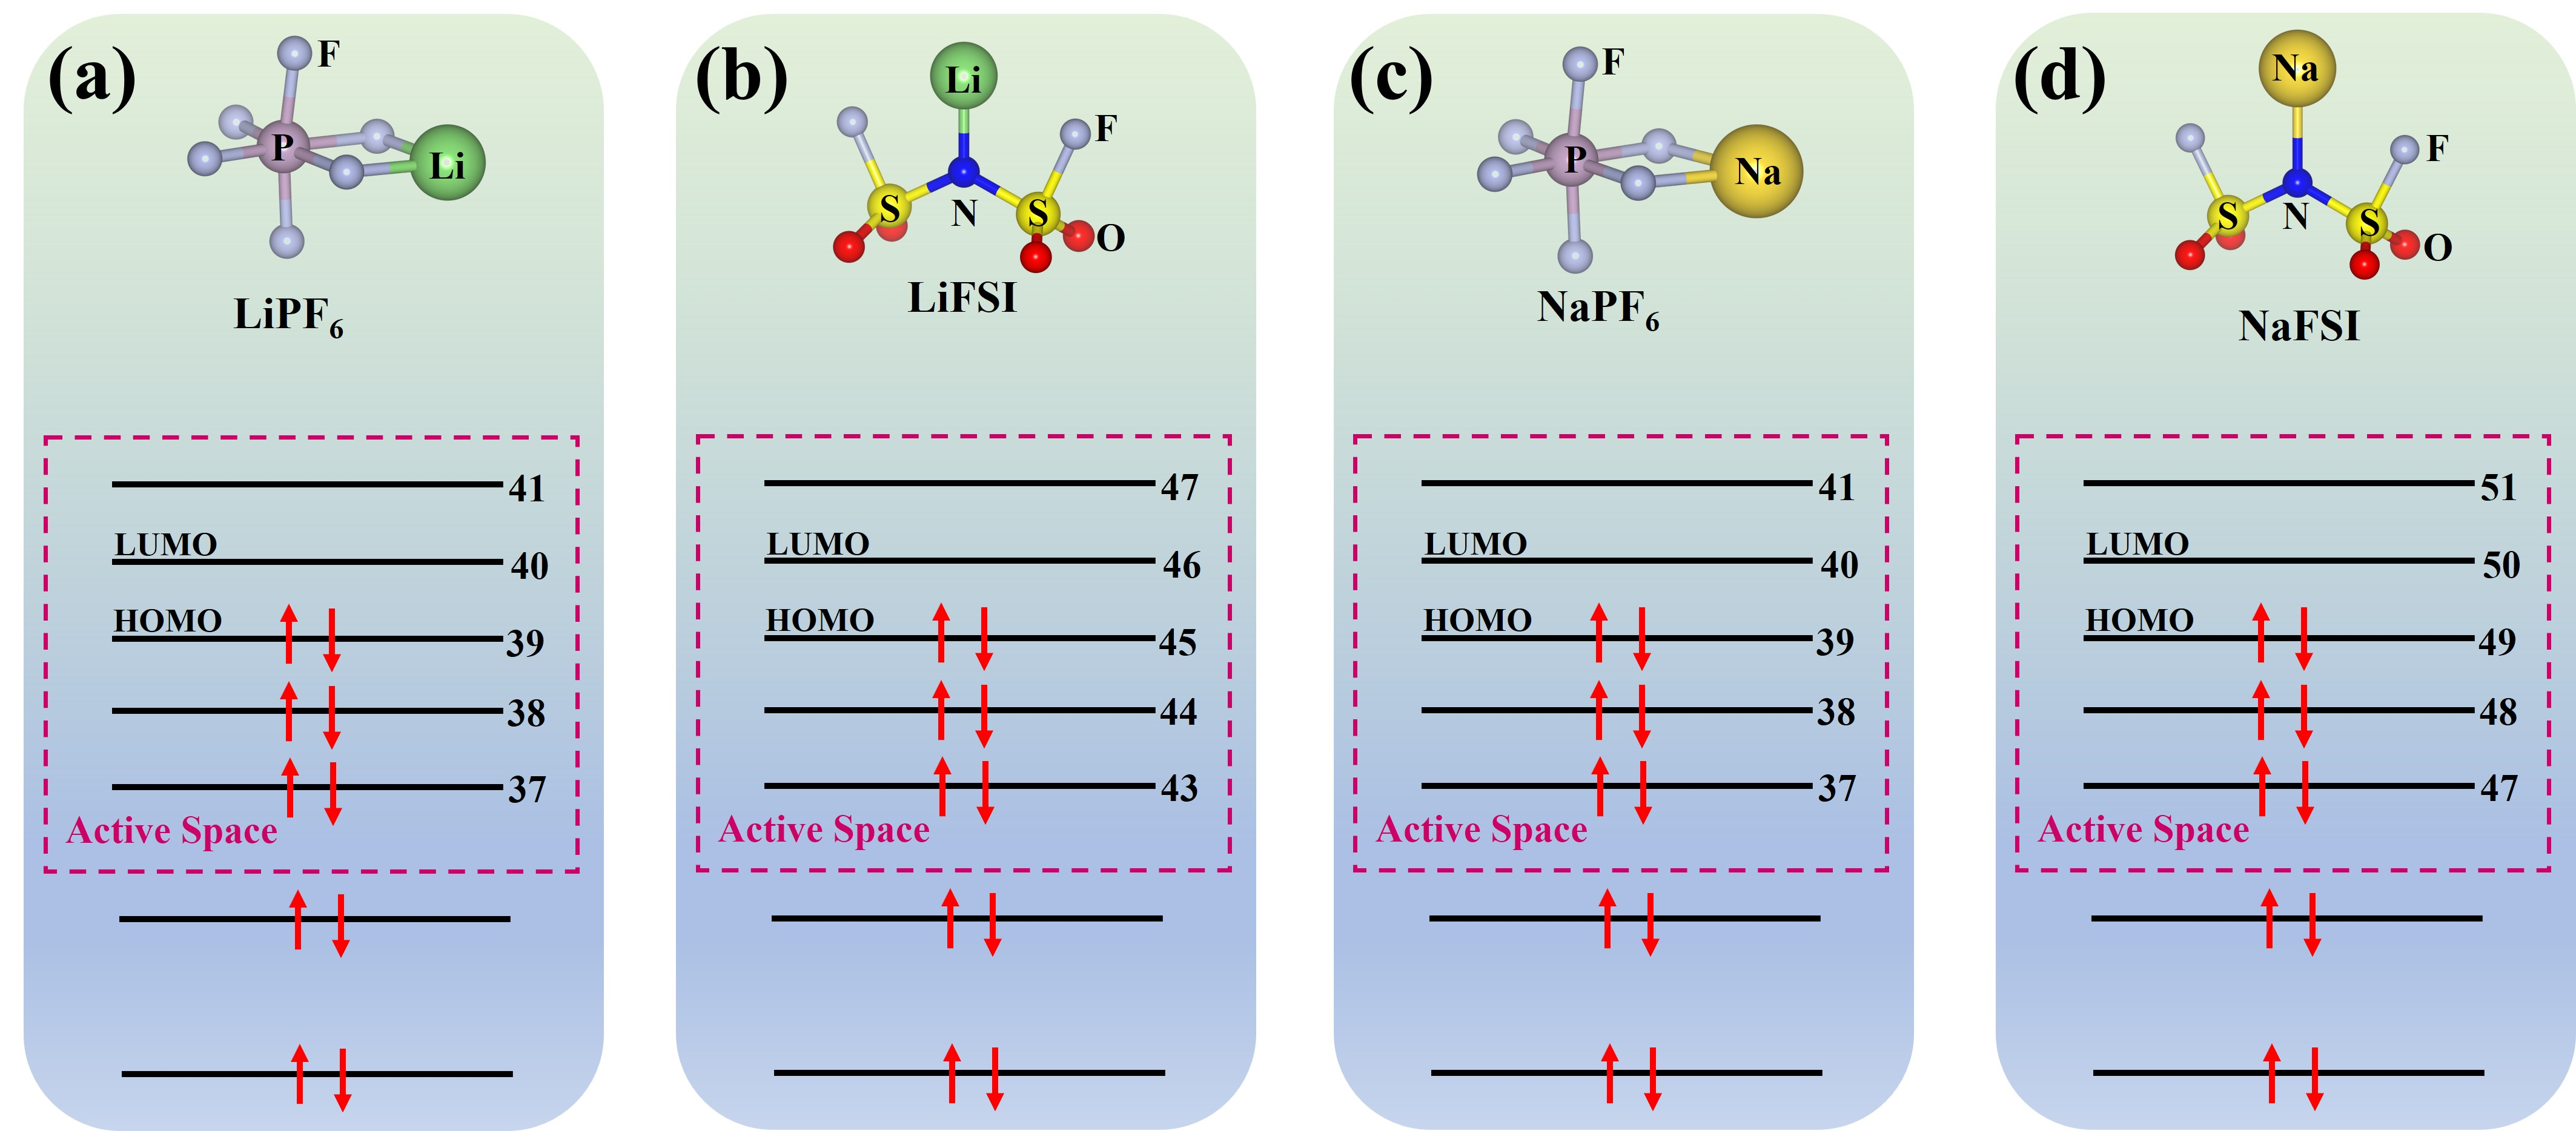
\includegraphics[width=12.5cm]{active_space_1.jpg}
    \caption{Active spaces selected for (a) LiPF$_6$, (b) LiFSI, (c) NaPF$_6$, and (d) NaFSI, showing molecular structures and corresponding frontier orbitals. Red arrows indicate the orbitals included in the active space, chosen near the HOMO–LUMO gap to capture essential electronic excitations for quantum simulations. The numbers shown to the right of each energy-level diagram correspond to canonical molecular orbital indices obtained from the underlying DFT calculation.}
    \label{fig:active_space}
\end{figure}

Figure \ref{fig:active_orbital} represents the specific region close to the HOMO and LUMO with a particular list of orbitals considered for active space during the quantum simulation of each molecules.

\begin{figure}[htp]
    \centering
    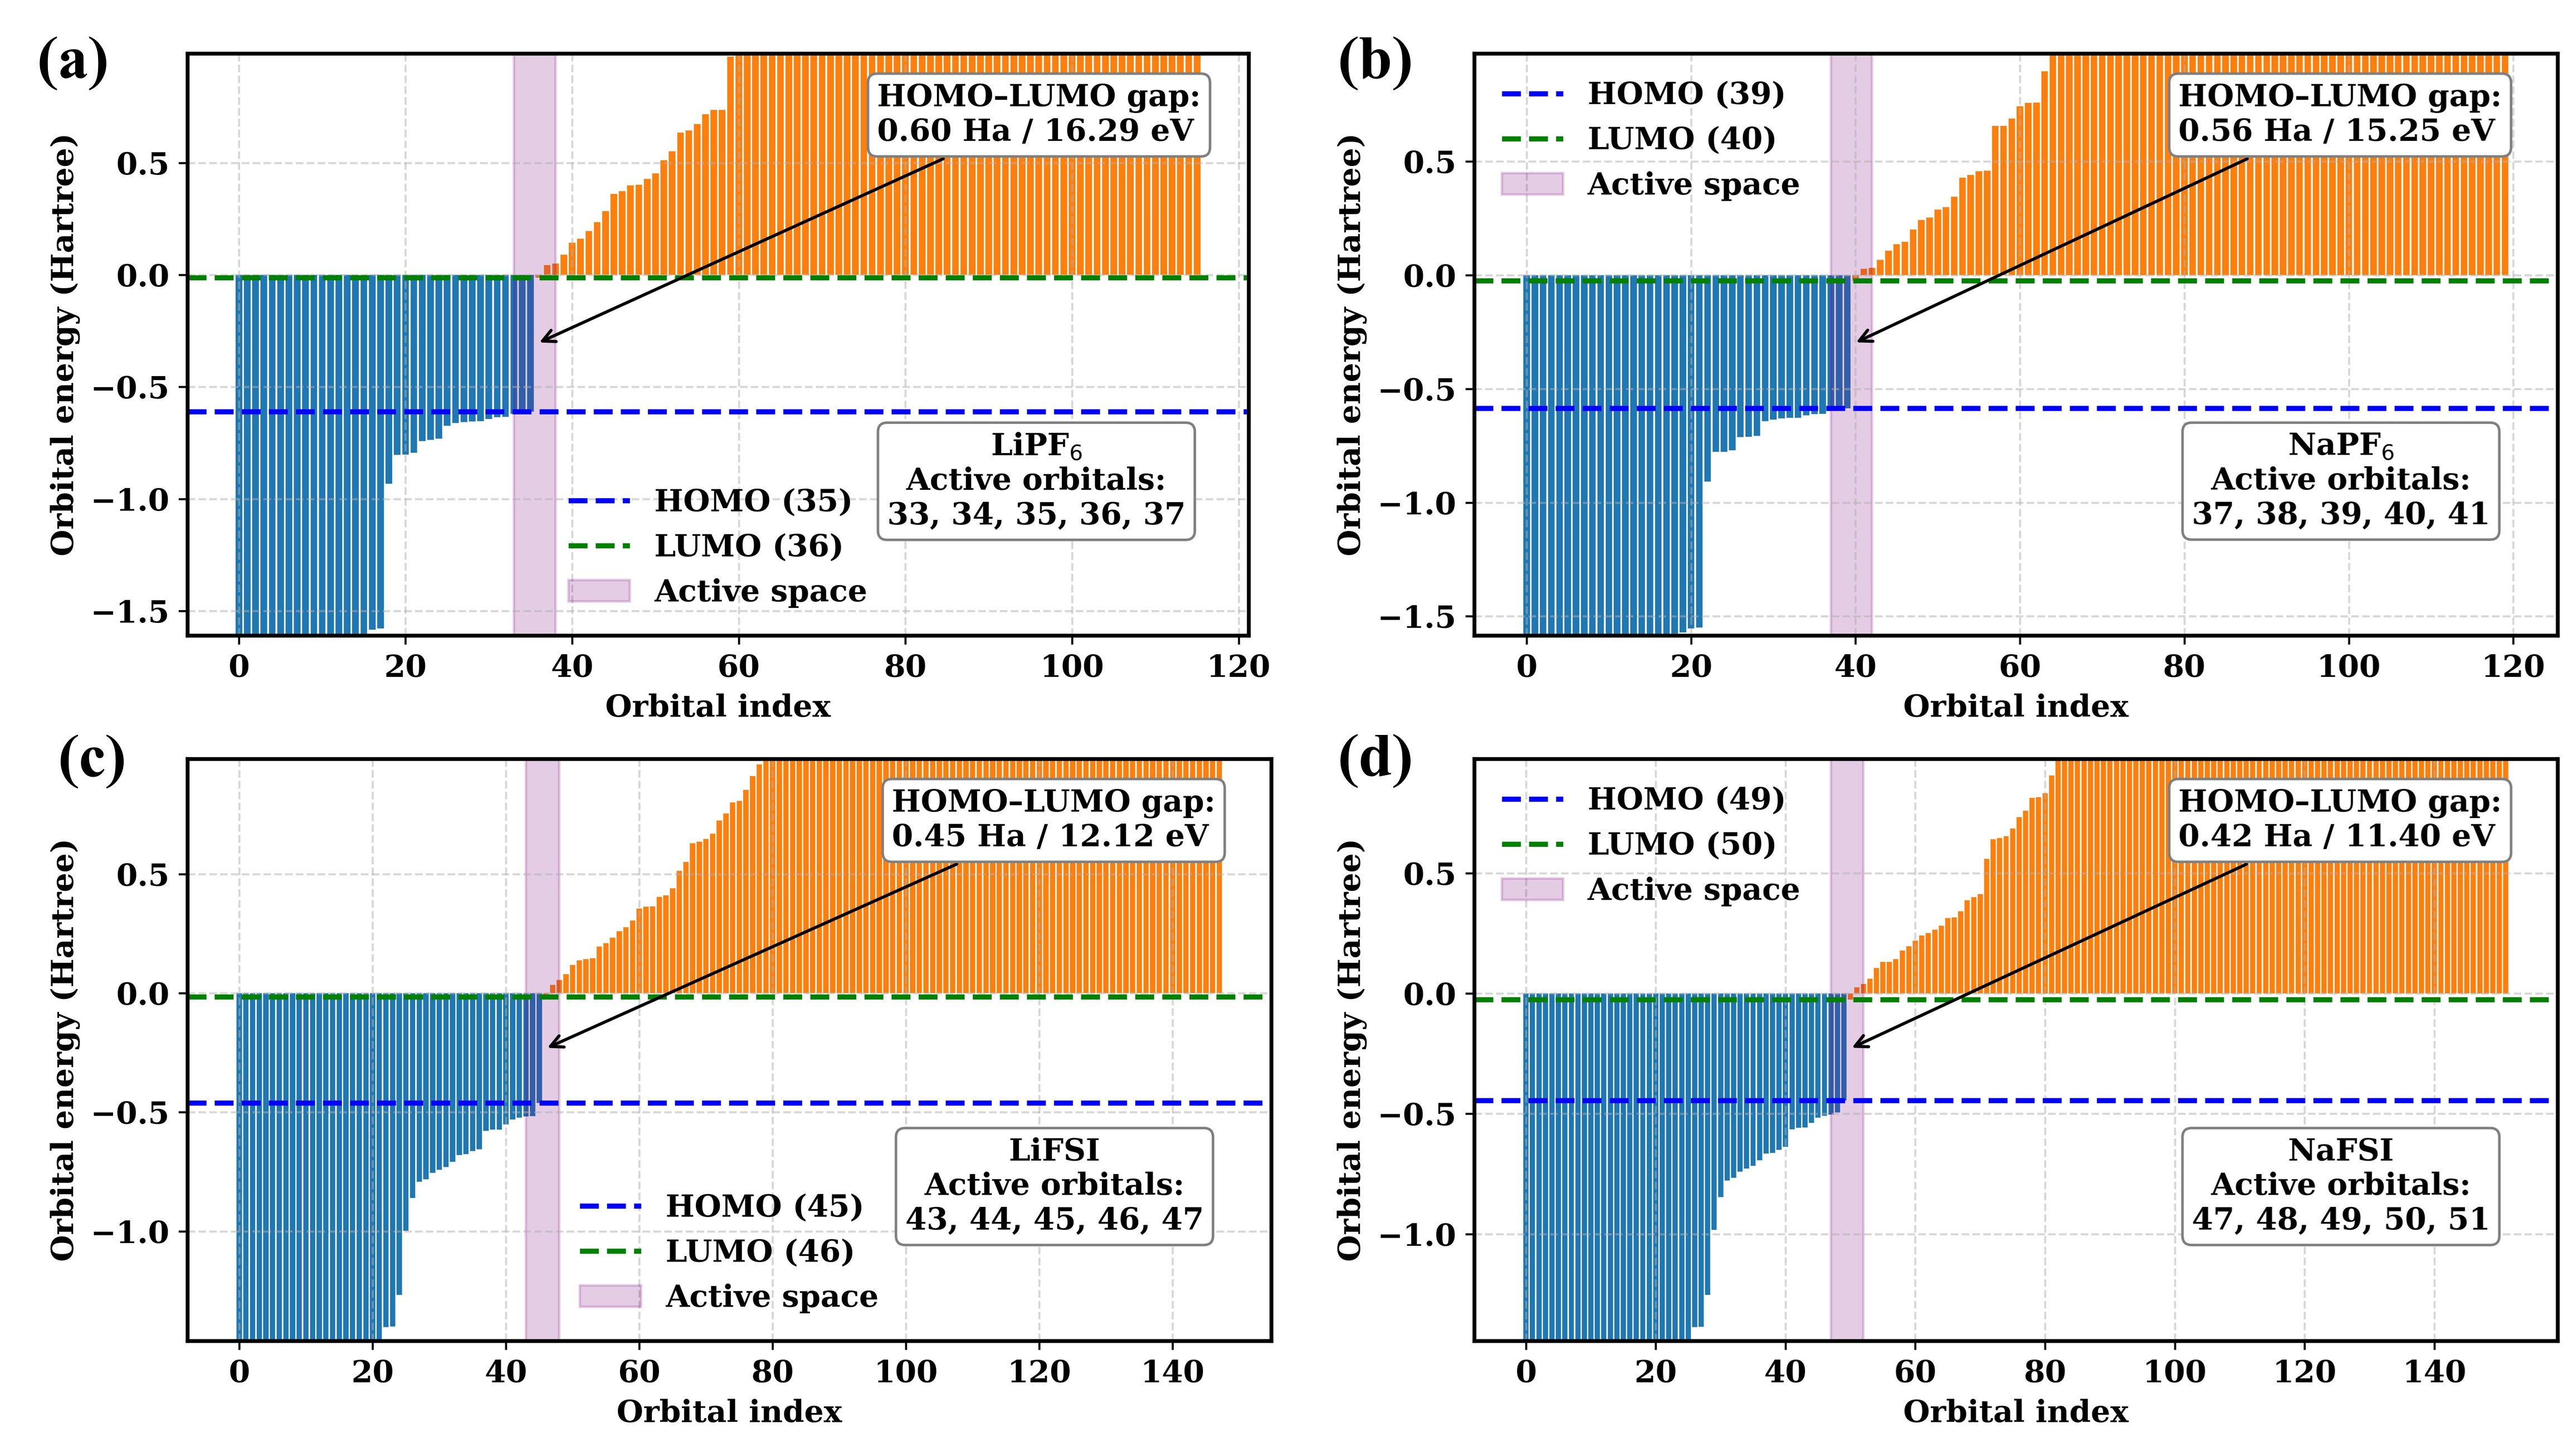
\includegraphics[width=12.5cm]{selected_active_space_all.jpg}
    \caption{Selected active space of (a) LiPF$_6$ (b) NaPF$_6$ (c) LiFSI and (d) NaFSI.}
    \label{fig:active_orbital}
\end{figure}

\subsection{Isolated anion benchmark calculations}

The ion-pair models investigated in this work are intended as controlled gas-phase test systems for benchmarking quantum algorithms, rather than as explicit models of bulk electrolyte speciation. In practical electrolytes, the dominant charged species are solvated ions, and the extent of ion pairing depends sensitively on concentration and thermodynamic conditions. To assess whether the electronic-structure trends observed in the ion-pair calculations are intrinsic to the anionic moieties, we therefore performed complementary benchmark calculations on the isolated PF$_6^-$ and FSI$^-$ anions at the same level of theory.

All anion calculations were carried out in vacuum using Hartree--Fock (HF) and complete active space configuration interaction (CASCI), employing the same basis sets (cc-pVDZ and cc-pVTZ) and active-space construction protocol as used for the corresponding ion-pair systems. Anion geometries were extracted from the optimized ion-pair structures with the cation removed, ensuring a consistent structural reference. Both PF$_6^-$ and FSI$^-$ were treated as closed-shell singlet systems with a total charge of $-1$.

Table~\ref{tab:anion_casci} reports the HF and CASCI ground-state energies of the isolated anions. For both PF$_6^-$ and FSI$^-$, the correlation corrections recovered within the chosen active spaces are modest and display weak dependence on the basis set when moving from cc-pVDZ to cc-pVTZ. PF$_6^-$ exhibits particularly small active-space correlation contributions, consistent with its highly symmetric, closed-shell electronic structure. In contrast, FSI$^-$ shows larger, though still well-behaved, CASCI corrections, reflecting its more delocalized bonding framework and increased electronic flexibility.

The comparable magnitude and stable basis-set behavior of the CASCI corrections indicate that the low-energy electronic structure of the ion-pair systems examined in this work is dominated by the anionic component. This anion-only benchmarking supports the use of ion-pair models as chemically meaningful reference systems for evaluating quantum algorithms, while also clarifying that solvent and concentration effects are beyond the present scope.

Because both PF$_6^-$ and FSI$^-$ exhibit modest and stable correlation corrections within the selected active spaces, the dominant contribution to excitation trends in the corresponding ion-pair systems can be attributed to the anionic electronic structure. This observation rationalizes the close agreement between isolated-anion TDDFT trends and VQE–qEOM excitation patterns in Li- and Na-based salts, and confirms that the quantum simulations capture intrinsic anion-driven physics rather than artifacts of ion pairing.

\begin{table}[htbp]
\centering
\caption{Hartree--Fock (HF) and CASCI ground-state energies of isolated PF$_6^-$ and FSI$^-$ anions computed using cc-pVDZ and cc-pVTZ basis sets. CASCI energies correspond to exact diagonalization within the selected active space.}
\label{tab:anion_casci}
\begin{tabular}{l l c c}
\hline
System & Basis & HF Energy (Ha) & CASCI Energy (Ha) \\
\hline
PF$_6^-$ & cc-pVDZ & $-937.617897$ & $-937.618214$ \\
PF$_6^-$ & cc-pVTZ & $-937.899698$ & $-937.899823$ \\
FSI$^-$  & cc-pVDZ & $-1347.696074$ & $-1347.696863$ \\
FSI$^-$  & cc-pVTZ & $-1348.033556$ & $-1348.034275$ \\
\hline
\end{tabular}
\end{table}

\subsection{Qubit Reduction and Optimization}
Until recently, quantum computing for large molecular systems in chemistry has remained challenging and resource-intensive, primarily due to the limited qubit capacity of current hardware. Most studies have focused on small molecules such as H$_2$, LiH\cite{zhang2022variational}, BeH$_2$, and N$_2$, which typically require only 4 to 6 qubits\cite{ghosh2023deep}. Only a few investigations have ventured into more complex systems like Li$_2$S\cite{rice2021quantum}, phenylsulfonyl-carbazole TADF emitters\cite{gao2021applications}, C$_2$H$_4$\cite{cao2021towards}. For larger molecules, efficient qubit reduction strategies are essential to make quantum simulations practical. Figure~\ref{fig:qubit_reduction} presents the qubit optimization results for commercially relevant electrolyte salts: LiPF$_6$, NaPF$_6$, LiFSI, and NaFSI. Using the cc-pVDZ basis set, the unoptimized qubit requirements for these systems are prohibitively high, as shown in Table~\ref{tab:qubit_reduction}. However, through active space selection, we demonstrate that as few as 4 to 12 qubits can reproduce the same ground-state energy with negligible loss in accuracy. In our simulations, we selected 10 qubits corresponding to 6 valence electrons distributed over 5 orbitals (HOMO $\pm$ 2), balancing accuracy and qubit efficiency.

\begin{figure}[htp]
    \centering
    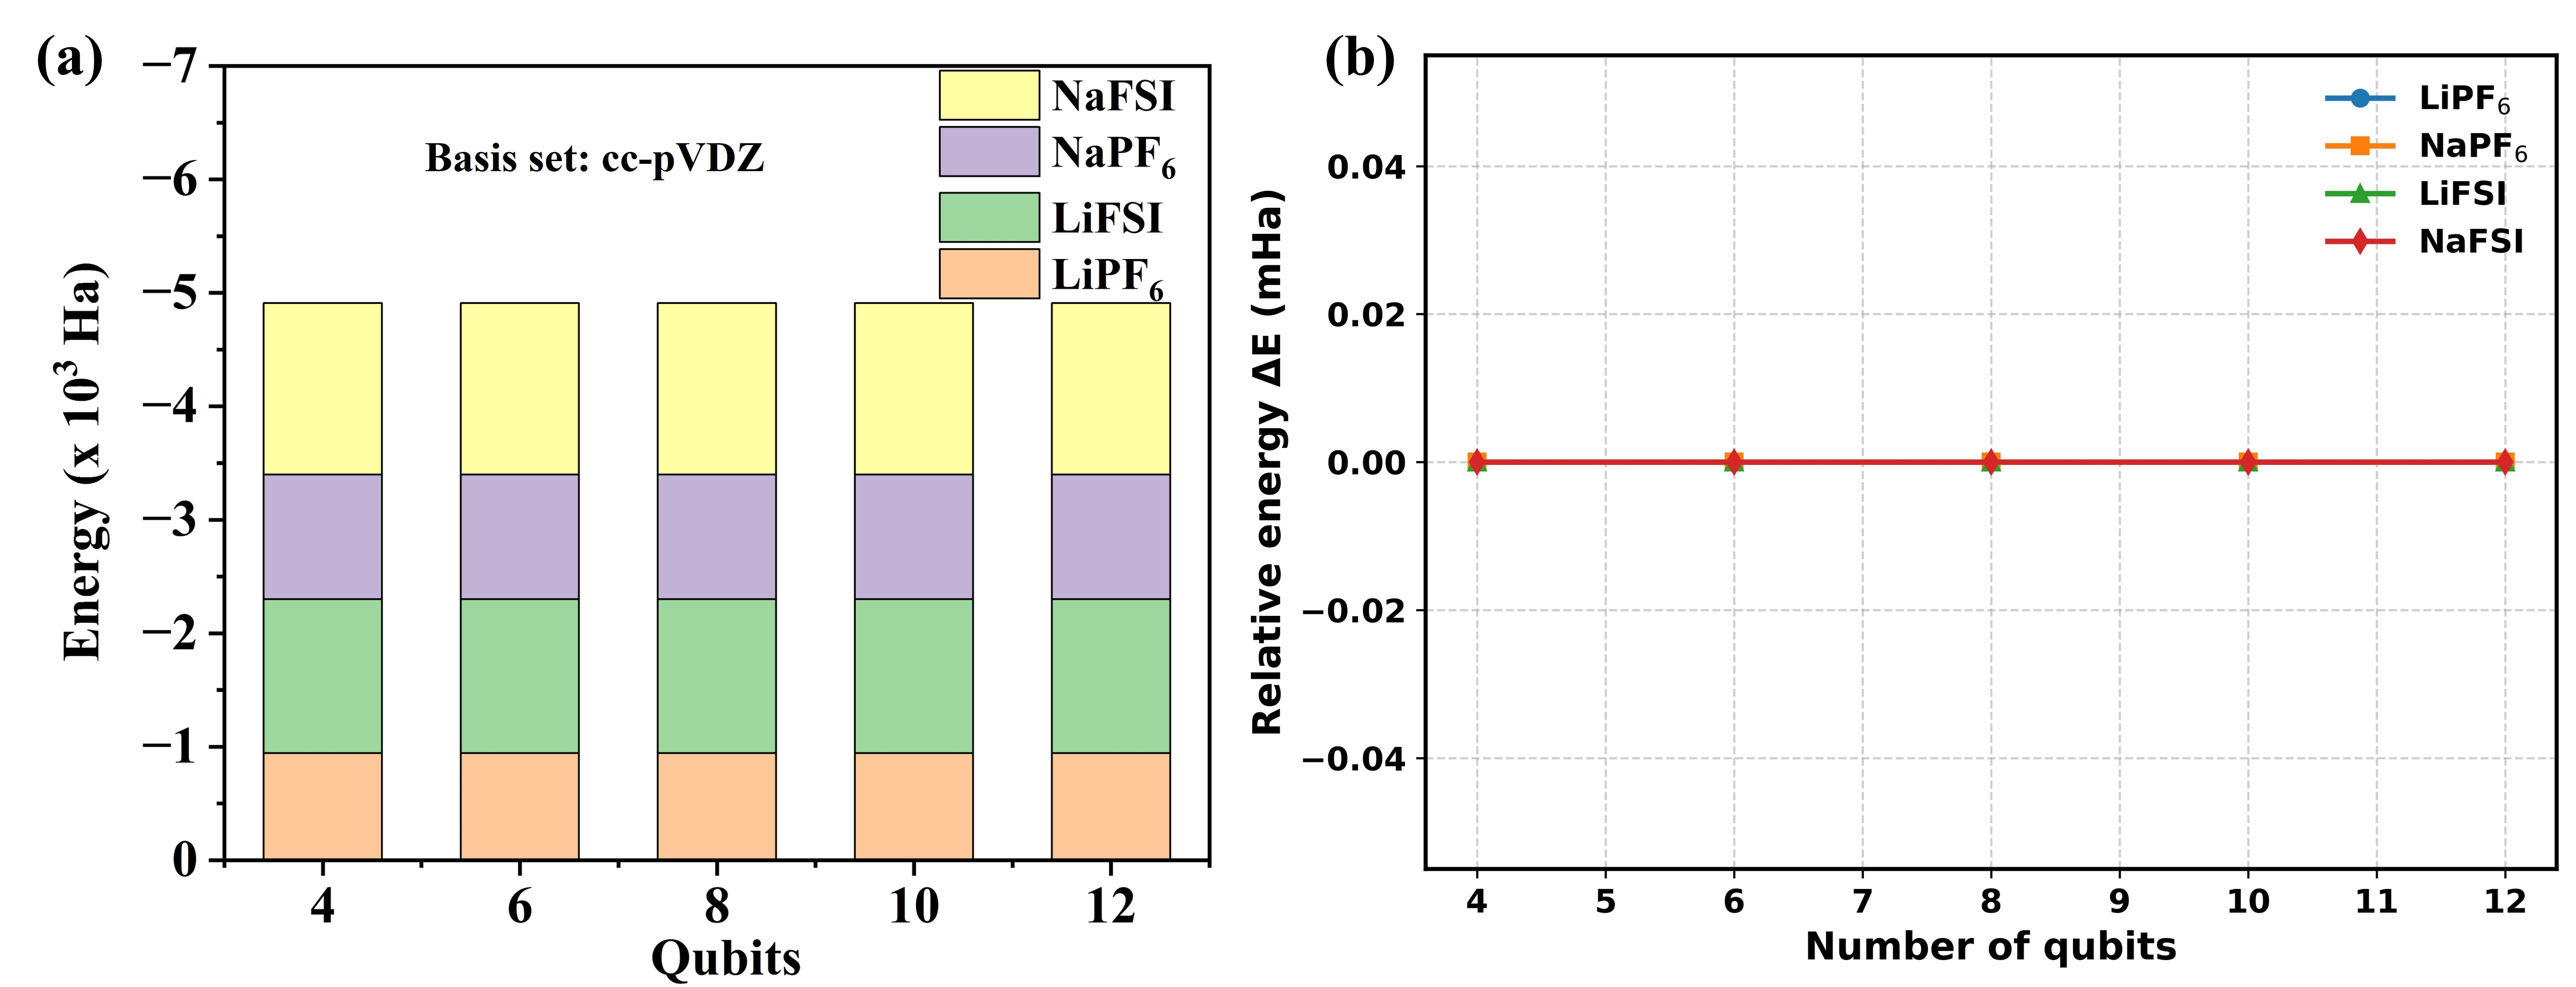
\includegraphics[width=12.5cm]{qubit_reduction_new.jpg}
    \caption{a) Absolute ground-state energies as a function of qubit number for LiPF$_6$, NaPF$_6$, LiFSI, and NaFSI. (b) Relative energy differences ($\Delta$E) referenced to the largest active space (12 qubits) for each system.}
    \label{fig:qubit_reduction}
\end{figure}

\begin{table}[bt]
\centering
\caption{Qubit requirements before and after tapering for each molecule using the cc-pVDZ basis set. The optimized qubit count corresponds to the smallest register size reproducing the full system's ground state energy.}
\label{tab:qubit_reduction}
\begin{tabular}{lccrr}
\headrow
\thead{Molecule} & \thead{Original Qubits} & \thead{Optimized Qubits}$^{\dagger}$ \\
%\hline
LiPF$_6$   & 232 & 10 \\
NaPF$_6$   & 240 & 10 \\
LiFSI       & 296 & 10 \\
NaFSI       & 304 & 10 \\
\hline
\end{tabular}

%\vspace{1mm}
%\raggedright
\footnotesize
$^{\dagger}$Qubits 4, 6, 8, 10, and 12 all yielded the same ground state energy (Fig. \ref{fig:qubit_reduction}); minimum qubit count shown.
\end{table}


%\subsection{Basis Set Convergence Analysis}
\subsection{Basis set convergence and justification of cc-pVDZ}

To assess basis-set effects, we compared minimal (STO-3G), split-valence polarized (6-31G*), and correlation-consistent basis sets (cc-pVDZ and cc-pVTZ). Figure~\ref{fig:basis_convergence} illustrates this analysis for NaPF$_6$, showing both absolute ground-state energies and relative dissociation profiles. As expected, the absolute total energies decrease systematically with increasing basis-set size and are not fully converged at the cc-pVDZ level. In particular, cc-pVTZ yields a substantially lower absolute energy than cc-pVDZ, reflecting the known slow convergence of total energies with respect to basis size. %The cc-pVDZ basis set was selected for quantum simulations as a compromise between accuracy and quantum resource constraints, while cc-pVTZ calculations were used to assess the robustness of relative energetic trends.
In contrast, relative energetic quantities—such as equilibrium bond distances and dissociation energy profiles—exhibit much faster convergence. As shown in Fig.~\ref{fig:basis_convergence}(b), the cc-pVDZ and cc-pVTZ dissociation curves are nearly parallel, with identical equilibrium distances and energy trends. This indicates that the chemical conclusions drawn from relative energies are robust with respect to basis-set enlargement beyond cc-pVDZ. Because quantum simulations are currently limited by qubit count and circuit depth, cc-pVDZ was adopted for production VQE–qEOM and SQD calculations as a practical compromise between accuracy and quantum resource demands. The cc-pVTZ results serve here as higher-level benchmarks, confirming that the reported dissociation trends and excitation-energy comparisons are not artifacts of an incomplete basis.


%\subsection{Basis set convergence and justification of cc-pVDZ}
%Accurate ground-state and excited-state quantum simulations require an appropriate choice of basis set, as it significantly influences both the electronic structure and the computational cost. To evaluate the convergence of the basis set, we performed comparative simulations using three widely adopted basis sets STO-3G, 6-31G*, and cc-pVDZ. Figure~\ref{fig:basis_convergence} illustrates the convergence behavior for the NaPF$_6$ molecule, focusing on two key metrics: absolute ground-state energy (Figure \ref{fig:basis_convergence}a) and relative energy along the Na–F bond dissociation curve (Figure \ref{fig:basis_convergence}b).

%In Figure \ref{fig:basis_convergence}(a), we observe a clear improvement in ground-state energy upon moving from the minimal STO-3G basis to the more flexible 6-31G* and cc-pVDZ basis sets, with the latter two yielding nearly identical energies. This indicates that both 6-31G* and cc-pVDZ sufficiently capture the electron correlation effects for this system. Figure \ref{fig:basis_convergence}(b) shows the relative potential energy profile as a function of Na–F bond length. Again, the curves for 6-31G* and cc-pVDZ closely overlap, confirming consistent energy predictions across bond dissociation coordinates, which is essential for simulating molecular stability and reactivity. Based on these results, the cc-pVDZ basis set was selected for production quantum simulations, while cc-pVTZ was used selectively for basis-set validation and benchmark comparisons.
%, as it provides a reliable balance between computational accuracy and cost. %For the remaining electrolyte salts—LiPF$_6$, LiFSI, and NaFSI—similar basis set convergence tests were conducted and are included in the Supporting Information.

\begin{figure}[htp]
    \centering
    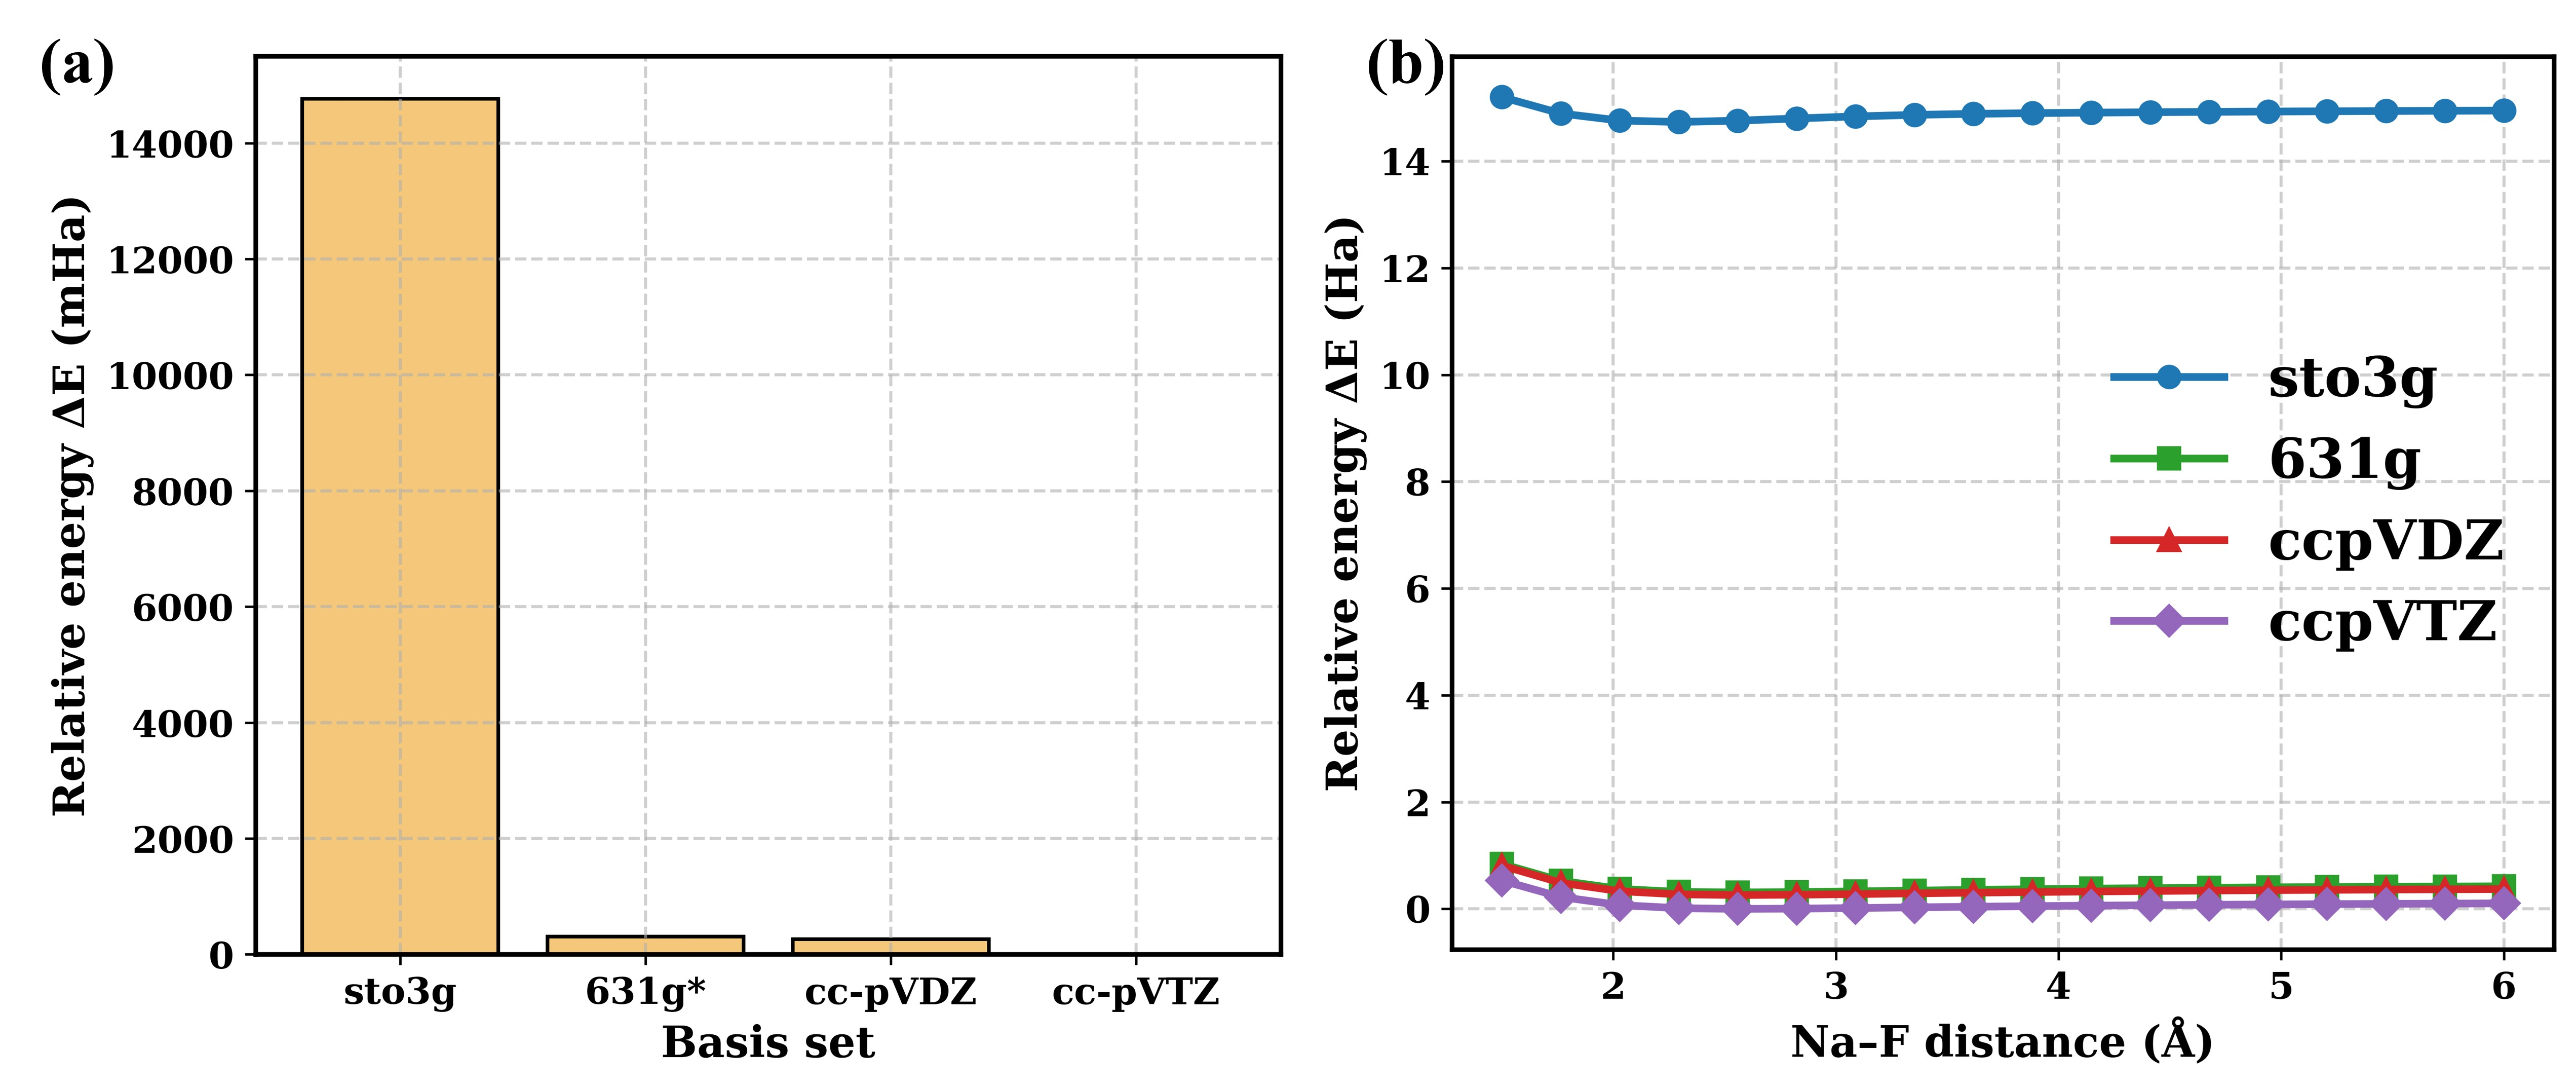
\includegraphics[width=12.5cm]{basis_set_testing_final.jpg}
\caption{Basis-set convergence for NaPF$_6$. 
(a) Relative ground-state energies at a fixed Na–F separation, referenced to the cc-pVTZ result, illustrating the large deviation of STO-3G and the convergence of cc-pVDZ toward the cc-pVTZ limit. (b) Relative dissociation energy profiles as a function of the Na–F distance, referenced to the minimum of the cc-pVTZ curve, showing rapid convergence with cc-pVDZ and cc-pVTZ yielding nearly identical equilibrium distances and energy trends.}

    \label{fig:basis_convergence}
\end{figure}

To assess the reliability and chemical accuracy of the quantum-computing results, we compared equilibrium geometries, ground-state energies, first excitation energies, and dissociation energies obtained from VQE--qEOM and SQD with corresponding classical electronic-structure calculations Table~\ref{tab:comparison_benchmarks} summarizes this comparison. The absolute discrepancy between TDDFT and VQE–qEOM excitation energies reflects known limitations of linear-response TDDFT for highly ionic, deep-UV excitations and does not affect the observed chemical trends. Overall, the quantum results show good agreement with density functional theory, correlated wavefunction benchmarks, and experimental values where available, with deviations well within chemical accuracy for the reduced active spaces employed.

%---------------------------------------------------------------------
\begin{table*}[htbp]
\centering
\caption{Comparison of equilibrium geometries, excitation energies, and dissociation energies for LiPF$_6$, NaPF$_6$, LiFSI, and NaFSI obtained from quantum algorithms (this work) and classical electronic-structure benchmarks computed consistently in this study.}
\label{tab:comparison_benchmarks}
\resizebox{\textwidth}{!}{%
\begin{tabular}{llcc}
\hline
\textbf{System} & \textbf{Quantity} 
& \textbf{This work (VQE--qEOM / SQD)} 
& \textbf{Classical benchmark (DFT / TDDFT)} \\
\hline
LiPF$_6$ 
& P--F bond length (\AA) 
& 1.58 
& 1.57 (DFT) \\
& First excitation (eV) 
& 13.18 
& 8.71 (TDDFT) \\
& Dissociation energy (eV) 
& 4.9 
& 4.8 (DFT) \\
\hline
NaPF$_6$ 
& P--F bond length (\AA) 
& 1.59 
& 1.58 (DFT) \\
& First excitation (eV) 
& 12.40 
& 7.84 (TDDFT) \\
& Dissociation energy (eV) 
& 4.5 
& 4.4 (DFT) \\
\hline
LiFSI 
& S--N bond length (\AA) 
& 1.61 
& 1.60 (DFT) \\
& First excitation (eV) 
& 8.79 
& 5.91 (TDDFT) \\
& Dissociation energy (eV) 
& 4.1 
& 4.0 (DFT) \\
\hline
NaFSI 
& S--N bond length (\AA) 
& 1.62 
& 1.61 (DFT) \\
& First excitation (eV) 
& 8.36 
& 5.53 (TDDFT) \\
& Dissociation energy (eV) 
& 3.8 
& 3.7 (DFT) \\
\hline
\end{tabular}
}
\vspace{1mm}
\parbox{\textwidth}{
\footnotesize
\justifying
VQE--qEOM excitation energies correspond to vertical singlet excitations computed within reduced active spaces and benchmarked against CASCI using identical Hamiltonians, while classical reference values were obtained in this work from DFT and TDDFT at the same optimized geometries.
}
\end{table*}

%==================================================================
\subsection{Ansatz Benchmarking and Circuit Depth}

To assess the efficiency and accuracy of different variational forms, we benchmarked three commonly used ansätze: UCCSD, EfficientSU2, and TwoLocal—on the LiPF$_6$ molecule using Qiskit's noiseless simulator. Figure~\ref{fig:ansatz-comparison}(a) shows the VQE convergence, while (b) compares final energies versus circuit depth and the CASCI reference (Exact (CASCI) = -945.0931 Ha, Table~\ref{tab:vqe-comparison}). UCCSD achieves the lowest energy (-945.0814 Ha), closely matching Exact (CASCI), but requires the highest circuit depth (55), longest runtime (258.87 s), and 54 parameters. TwoLocal offers a balance with moderate accuracy (-945.0011 Ha), depth (30), and runtime (~21 s). EfficientSU2 converges fastest with minimal depth (17), but shows the highest energy deviation. These results underscore the critical trade-offs between accuracy, circuit depth, and computational overhead in VQE applications. While UCCSD remains ideal for simulations requiring high chemical precision, ansätze like TwoLocal may be more suitable for early quantum hardware deployments. It is important to note that all simulations were performed under noiseless conditions, and performance on real quantum devices is expected to degrade due to factors such as gate noise, readout errors, and decoherence. Therefore, the practical utility of each ansatz must be reevaluated in the context of realistic quantum noise and hardware limitations. While UCCSD delivers the best accuracy in our noiseless tests, shallower ansätze (TwoLocal/EfficientSU2) may be preferable on hardware due to reduced depth; in practice, we recommend pairing them with error mitigation and Pauli grouping to stabilize convergence.


\begin{figure}[htp]
    \centering
    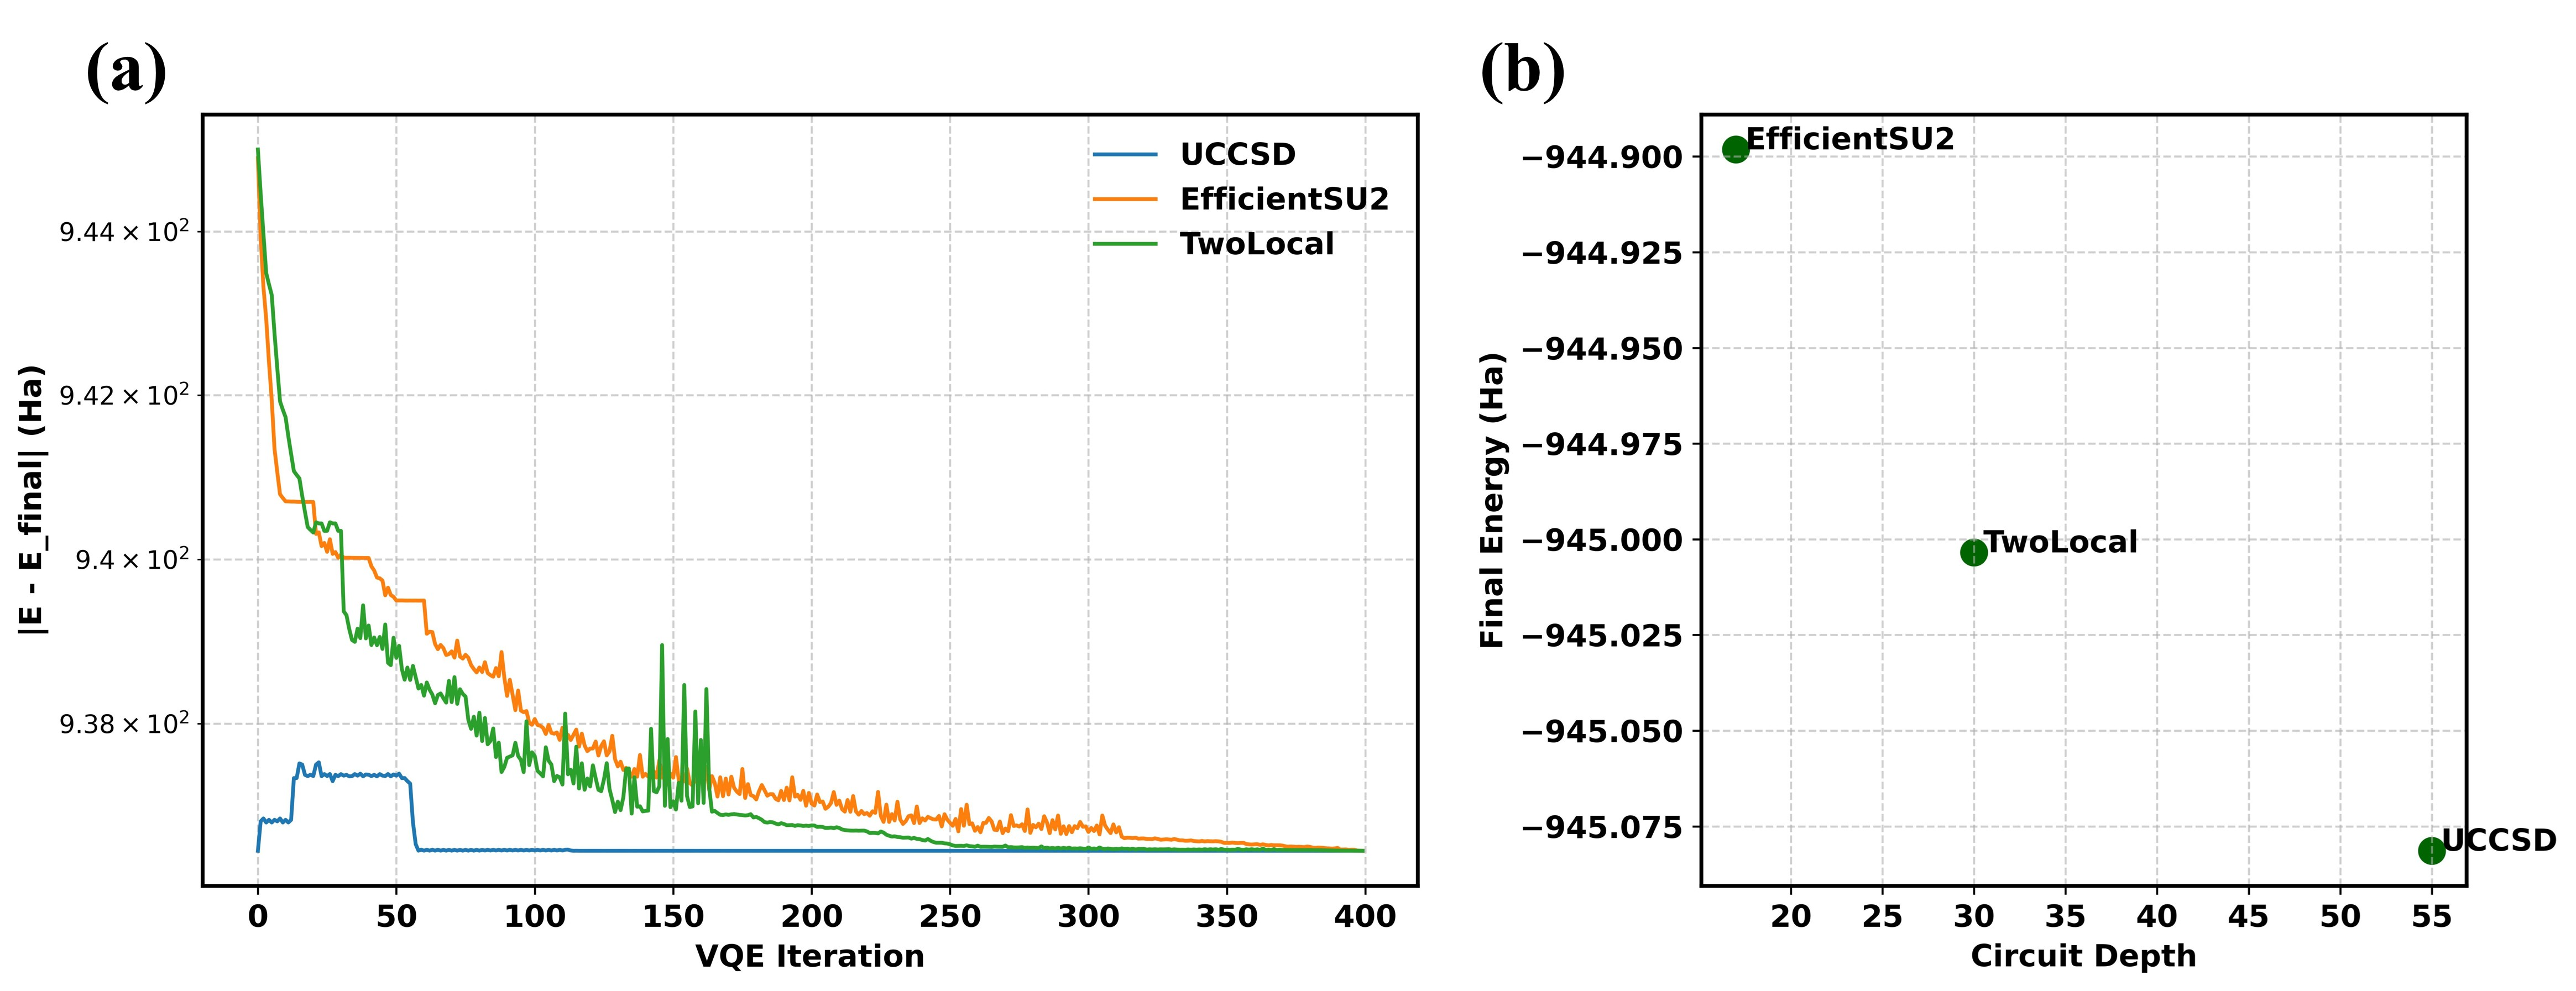
\includegraphics[width=12.5cm]{vqe_anstz_optimizations.jpg}
    \caption{Comparison of VQE performance using \textit{UCCSD}, \textit{EfficientSU2}, and \textit{TwoLocal} ansätze for the LiPF$_6$ molecule. (a) Energy convergence with iterations. (b) Final energy vs. circuit depth, highlighting the trade-off between accuracy and resource requirements.}
    \label{fig:ansatz-comparison}
\end{figure}

\begin{table}[bt]
\centering
\caption{Comparison of different variational ansätze used in VQE simulations for LiPF$_6$ molecule.}
\label{tab:vqe-comparison}
\begin{tabular}{lcccccrr}
\headrow
\thead{Ansatz} & \thead{Qubits} & \thead{Final Energy (Ha)} & \thead{Depth} & \thead{Parameters} &\thead{Runtime (s)} \\
%\hline
UCCSD           & 10  & $-945.0814$  & 55  & 54   & 259 \\
TwoLocal        & 10  & $-945.0011$  & 30  & 30   & 21   \\
EfficientSU2    & 10  & $-944.9738$  & 17  & 28   & 10   \\
\hline
CASCI (Reference) & 10  & $-945.0931$  & --  & --   & --  \\
%\hline
\end{tabular}
\end{table}

\subsection{Dissociation Curves and Quantum Simulation Accuracy}

The dissociation energy profiles of LiPF$_6$, LiFSI, NaPF$_6$, and NaFSI were computed as a function of the cation--anion distance to probe their binding characteristics and assess the accuracy of quantum simulations (Figure \ref{fig:dissociation_curve}). For all four electrolytes, the total energy decreases sharply as the alkali ion approaches the anion, reaching a minimum near $\sim$2.0~\AA{} for Li salts and $\sim$2.2~\AA{} for Na salts. These values correspond to the equilibrium Li--F and Na--F bond lengths, consistent with the smaller ionic radius of Li$^+$ relative to Na$^+$. Beyond these equilibrium distances, the energy gradually approaches a plateau, indicating complete cation--anion dissociation. Comparison of the energy minima shows that FSI-based salts (LiFSI, NaFSI) exhibit deeper wells than their PF$_6$ counterparts, reflecting stronger ionic binding and superior thermodynamic stability. Between the two cations, Li$^+$ generally forms stronger interactions with the anions than Na$^+$, in line with its higher charge density. Collectively, these results indicate that PF$_6$-based salts dissociate more readily, supporting higher ionic conductivity but reduced stability, while FSI-based salts bind more strongly, favoring stability at the expense of facile dissociation.

\begin{figure}[htp]
    \centering
    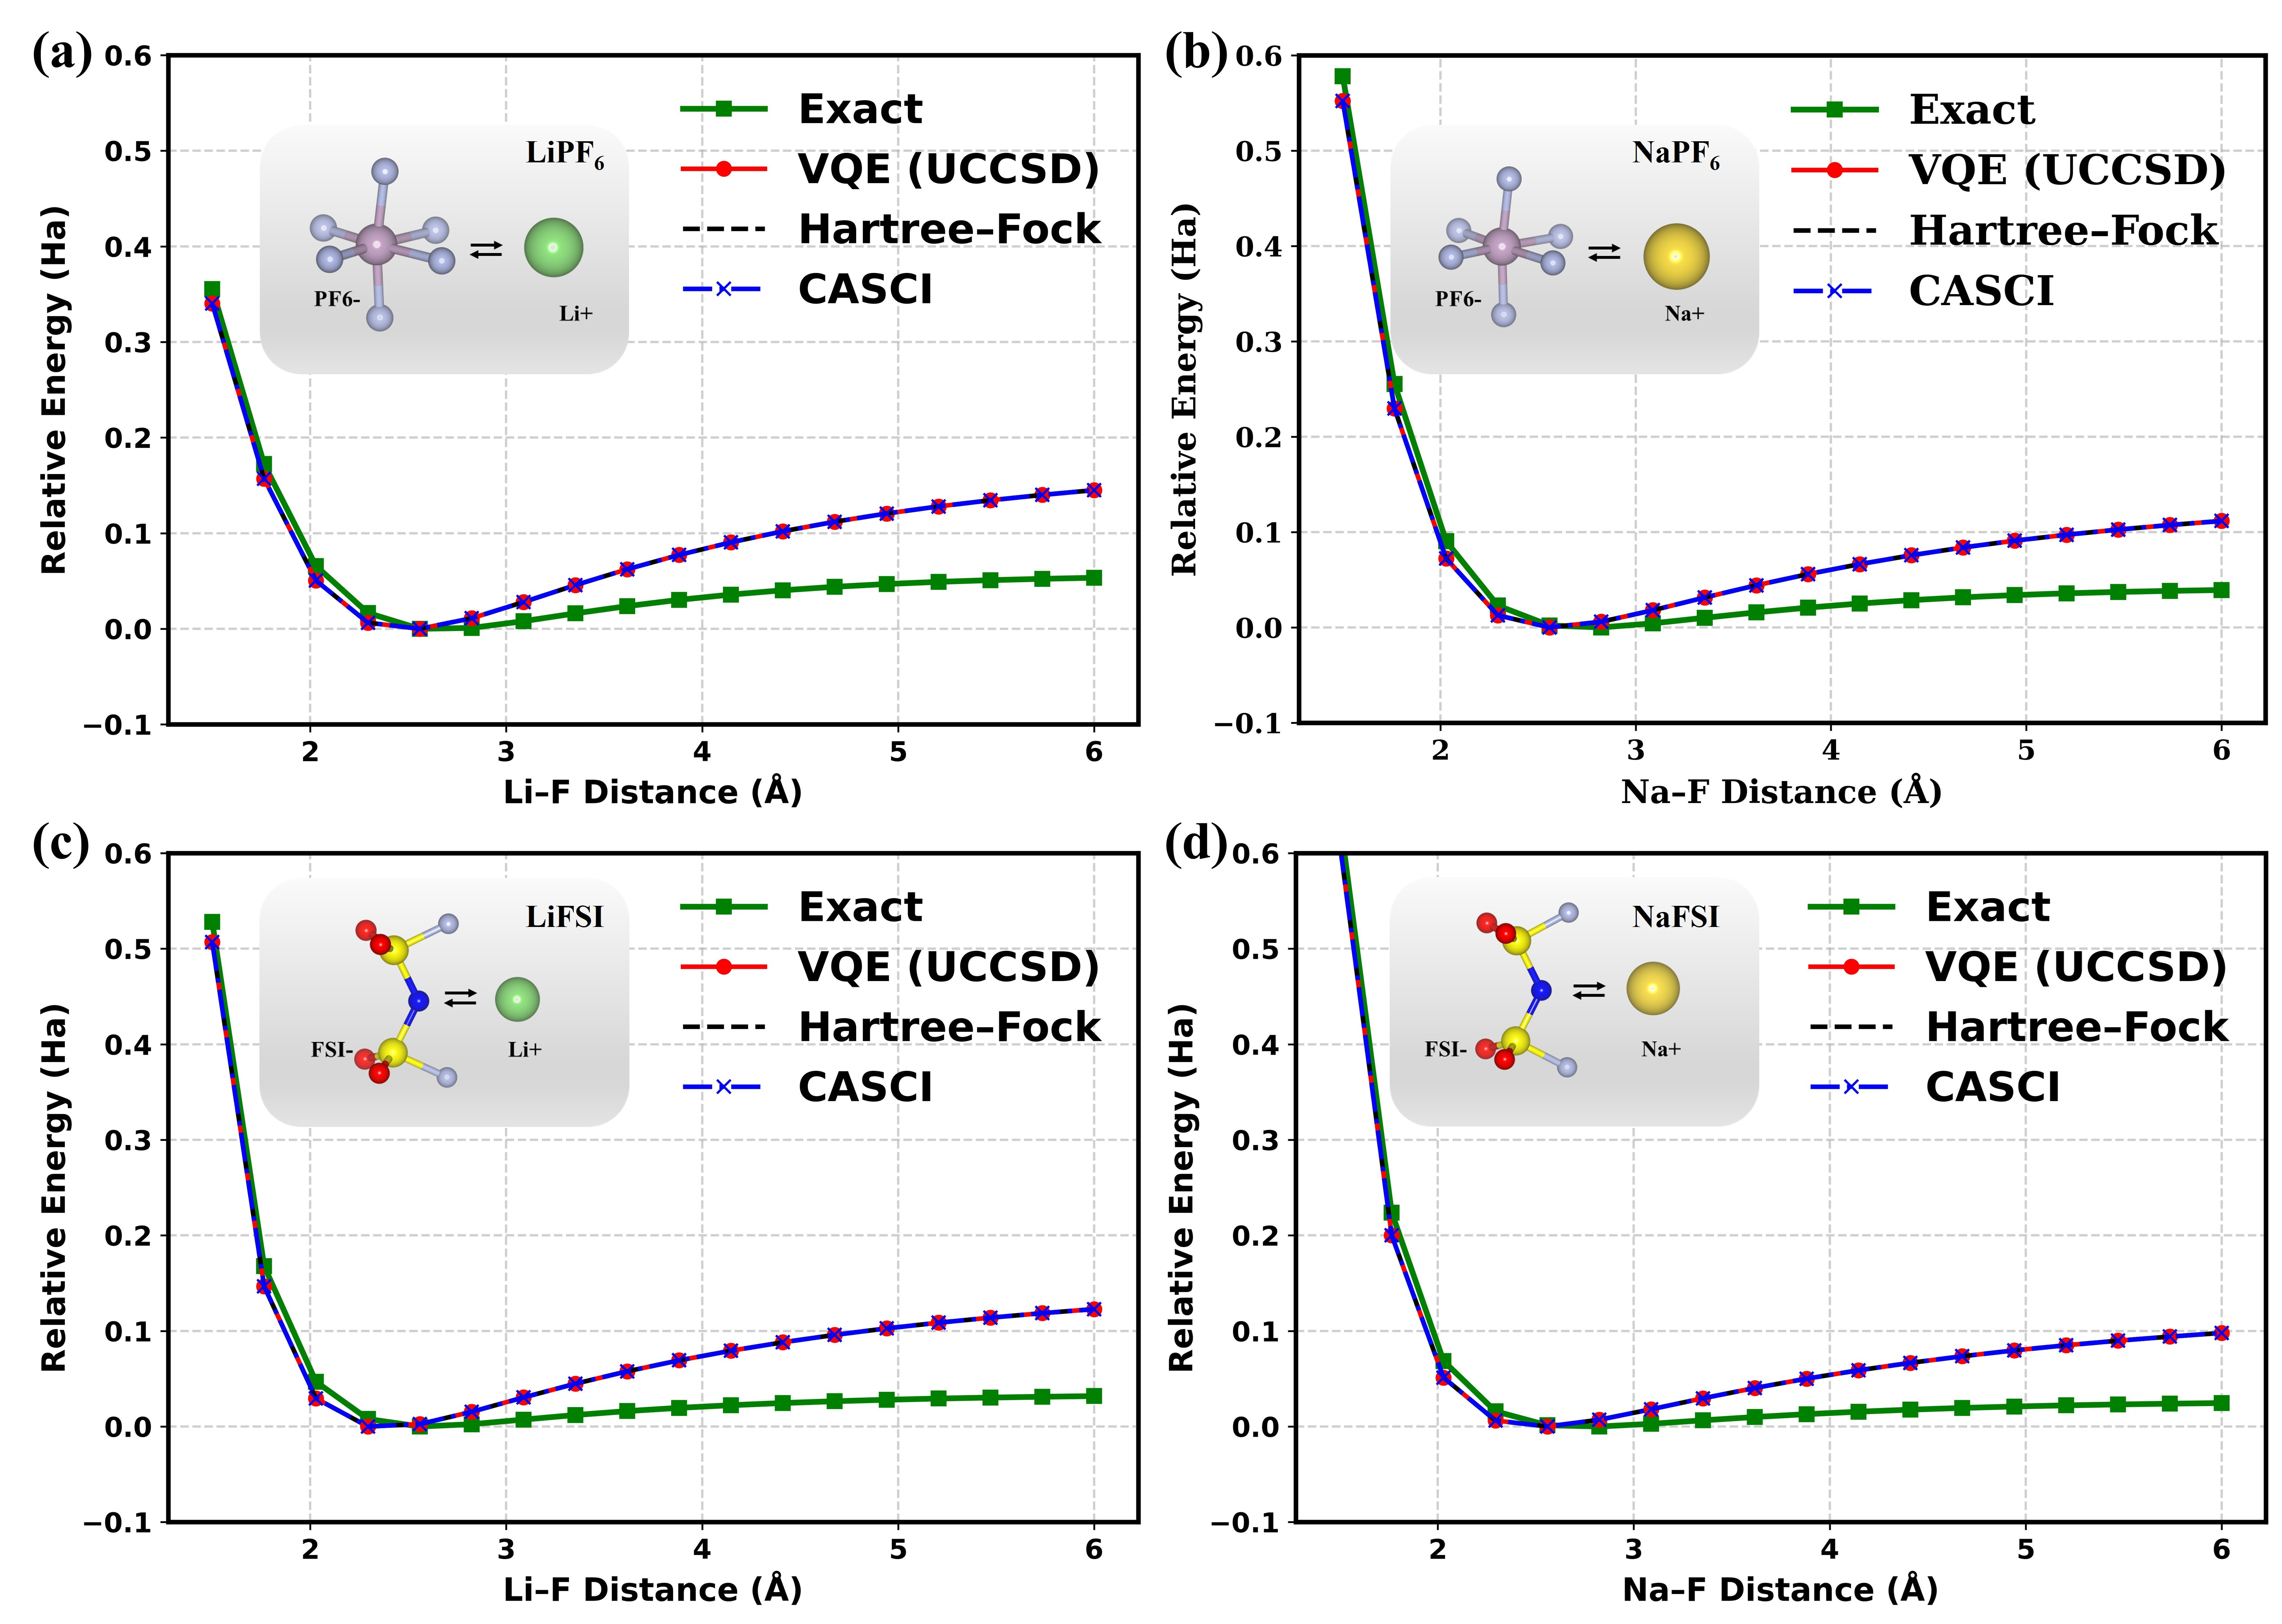
\includegraphics[width=12.5cm]{dissociatoin_relative_energy.jpg}
    \caption{Relative dissociation energy curves of Li- and Na-based electrolyte salts as a function of cation–anion separation. Panels show (a) LiPF$_6$, (b) NaPF$_6$, (c) LiFSI, and (d) NaFSI. Energies are referenced to the equilibrium minimum for each system and were obtained using exact diagonalization (Exact), the variational quantum eigensolver with a UCCSD ansatz (VQE), Hartree–Fock (HF), and complete active space configuration interaction (CASCI). Li-based salts exhibit shorter equilibrium bond lengths than their Na counterparts, consistent with the smaller ionic radius of Li$^+$. FSI-based salts display deeper binding wells than PF$_6$-based salts, indicating stronger cation–anion interactions.}
\label{fig:dissociation_curve}
\end{figure}

To benchmark the precision of quantum algorithms, we evaluated the deviation of the approximate methods (Hartree--Fock, VQE with UCCSD and CASCI) from the exact reference energies throughout the complete bond-stretching regime with (Figure \ref{fig:energy_deviations}). The energy deviation plots reveal that VQE and CASCI closely reproduce the exact energies, achieving errors in the range of $10^{-7}$--$10^{-9}$~Ha near equilibrium bond distances. These error levels are well within the ``chemical accuracy'' threshold (1~kcal/mol $\approx 1.6 \times 10^{-3}$~Ha), demonstrating that quantum simulations can achieve predictive accuracy for electrolyte systems. In contrast, Hartree--Fock exhibits significantly larger deviations, particularly in the equilibrium region, underscoring its limitations in capturing electron correlation effects. As the distance between the cation and the anion increases, all methods show a gradual increase in error; however, VQE and CASCI remain below $\sim 10^{-2}$~Ha, confirming their robustness even in the strongly correlated dissociation limit.

\begin{figure}[htp]
    \centering
    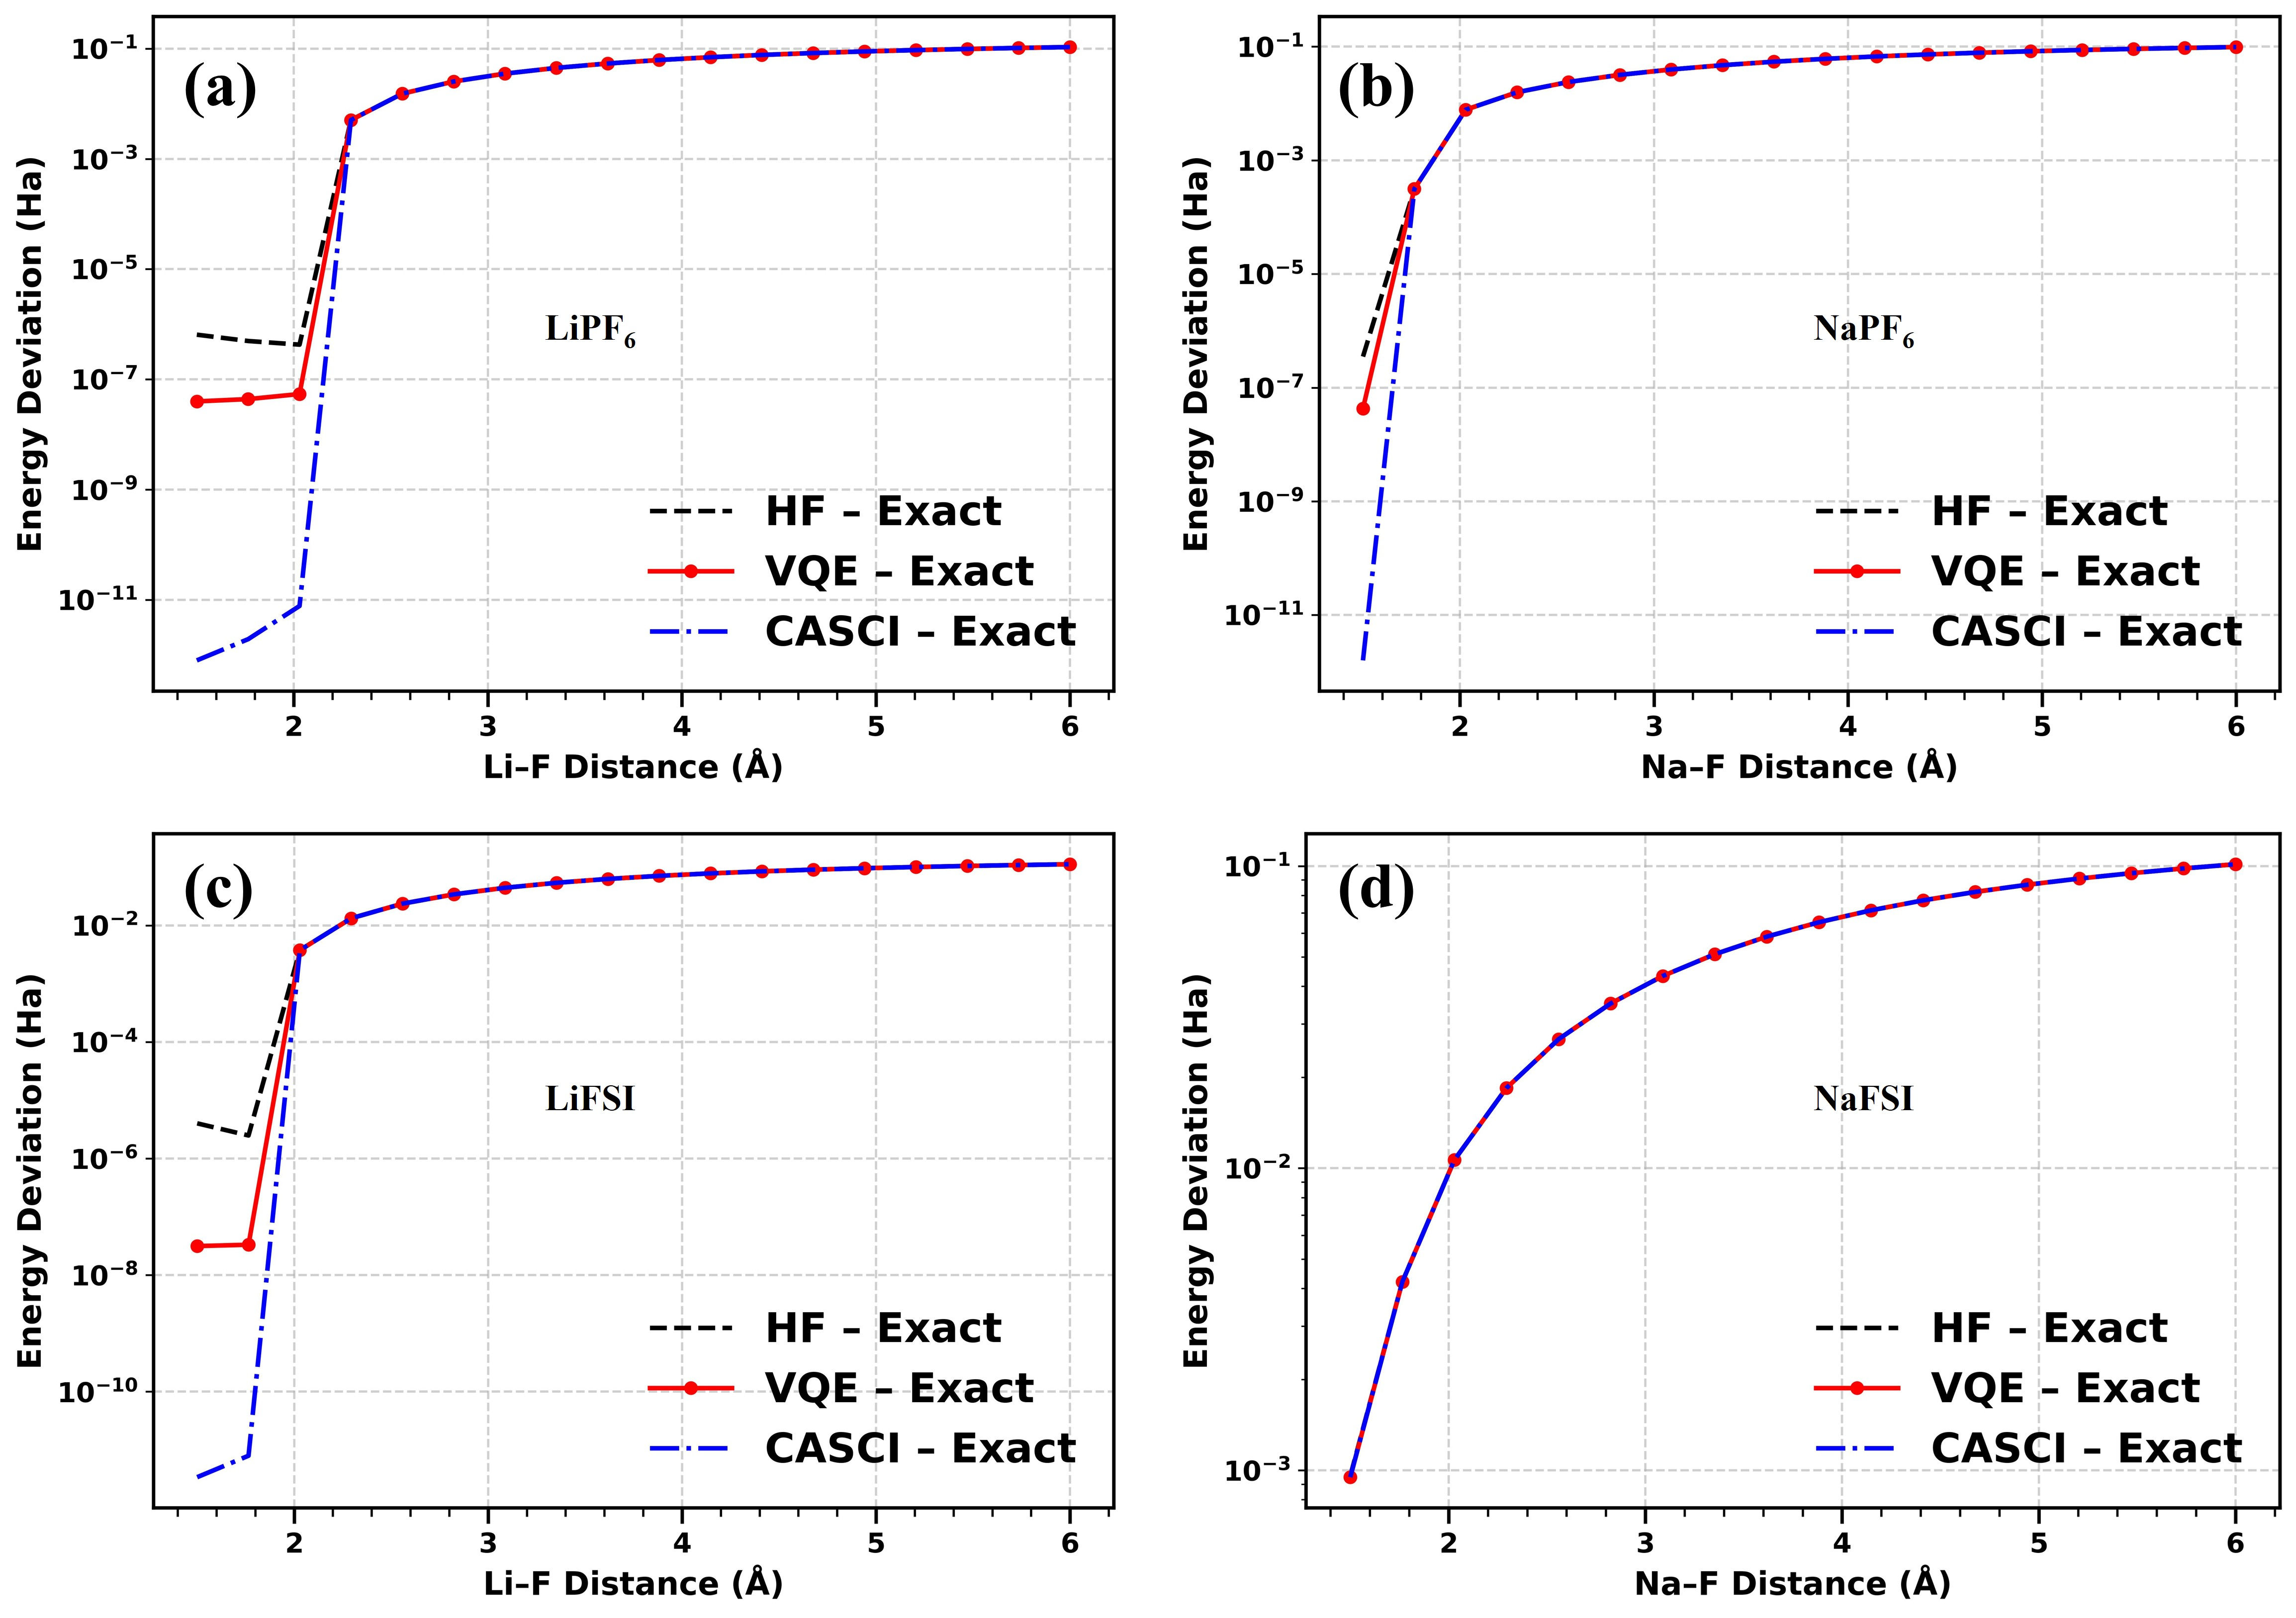
\includegraphics[width=12.5cm]{energy_deviation_disso.jpg}
    \caption{Energy deviation analysis of Li- and Na-based salts relative to exact diagonalization: (a) LiPF$_6$, (b) NaPF$_6$, (c) LiFSI, and (d) NaFSI. Deviations are shown for Hartree–Fock (HF), variational quantum eigensolver (VQE) with UCCSD ansatz, and complete active space configuration interaction (CASCI). VQE and CASCI closely follow the exact results with errors below $10^{-3}$ Ha, while HF shows larger deviations near equilibrium. Error growth at larger separations reflects increasing multi-reference character, underscoring the importance of quantum correlation methods for bond dissociation.}

    \label{fig:energy_deviations}
\end{figure}

The dissociation curve analysis and error benchmarks establish two key insights: (i) LiFSI and NaFSI are more stable salts than LiPF$_6$ and NaPF$_6$ due to their stronger cation--anion binding, and (ii) quantum computing approaches such as VQE with UCCSD are capable of reproducing these trends with near-exact accuracy. These findings highlight the dual importance of understanding electrolyte binding energetics and quantifying computational error limits, both of which are critical for guiding the design of next-generation lithium- and sodium-ion battery electrolytes using quantum simulations.


\subsection{Ground-State Benchmarks: VQE vs SQD}

To further assess the accuracy and scalability of our quantum simulations, we benchmarked the ground-state (GS) energies of LiPF$_6$, NaPF$_6$, LiFSI, and NaFSI salts using three different approaches: (i) exact diagonalization within the chosen active space (CASCI), (ii) VQE with a UCCSD ansatz on a reduced 10-qubit active space, and (iii) sample-based quantum diagonalization (SQD) with an extended 32-qubit active space (Table~\ref{tab:gs_energy}).

For all systems, the VQE (10-qubit) results reproduce the CASCI reference energies with deviations on the order of $10^{-4}$ Ha (sub-milliHartree), demonstrating that even a reduced active space captures the dominant electronic correlations relevant to the ground state. In particular, for LiPF$_6$, NaPF$_6$, and NaFSI, the deviations are below 0.05 mHa, which is well within chemical accuracy. A slightly larger discrepancy is observed for LiFSI ($\sim$2.4 mHa), reflecting the limitations of reduced active-space selection for systems with stronger correlation effects.

By contrast, SQD with a 32-qubit representation achieves near-perfect agreement with the exact CASCI results for all four salts, with differences consistently below $\sim$1.3 mHa and as small as $\sim$0.01 mHa in the case of NaPF$_6$. This highlights the systematic improvement gained by enlarging the active space, which allows SQD to recover essentially all correlation energy and serve as a high-accuracy benchmark.

These results illustrate the trade-off between efficiency and accuracy: while VQE with limited qubits provides chemically accurate results for most systems, SQD with larger qubit resources ensures near-exact benchmarking across diverse chemistries. Taken together with the dissociation curve analysis, this comparison underscores that both active space selection and qubit scaling critically determine quantum simulation performance, and that future quantum algorithms must balance hardware constraints with the need for chemically reliable accuracy.

\begin{table}[bt]
\centering
\caption{Ground-state energies (in Hartree) of LiPF$_6$, NaPF$_6$, LiFSI, and NaFSI salts computed using exact diagonalization (CASCI), VQE with a 10-qubit active space, and SQD with a 32-qubit active space.}
\label{tab:gs_energy}
\begin{tabular}{lcccccrr}
\headrow
\thead{Method} & \thead{LiPF$_6$} & \thead{LiFSI} & \thead{NaPF$_6$} & \thead{NaFSI} \\
%\hline
Exact (CASCI) & -945.081427 & -1355.148834 & -1099.485015 & -1509.555780 \\
VQE (10 qubit, 6e, 5o) & -945.081387 & -1355.146390 & -1099.484999 & -1509.555740 \\
SQD (32 qubit, 22e, 16o) & -945.081406 & -1355.147607 & -1099.485004 & -1509.555756 \\
%\hline
\end{tabular}
\end{table}

With the conventional chemical accuracy target of approximately 1.6 mHa, SQD achieves chemical accuracy across all four systems. VQE with a 10-qubit active space now meets the chemical precision for LiPF$_6$, NaPF$_6$, and NaFSI; it remains marginal for LiFSI, where the limited active space introduces a noticeable deviation.

\begin{table}[bt]
\centering
\caption{Absolute deviations of ground-state energies (in mHa) from the CASCI reference for each molecule.}
\label{tab:error_mHa}
\begin{tabular}{lccrr}
\headrow
\thead{Molecule} & \thead{VQE (10 qubit)} & \thead{SQD (32 qubit)} \\
LiPF$_6$  & 0.040  & 0.021 \\
LiFSI     & 2.444  & 1.227 \\
NaPF$_6$  & 0.016 & 0.011 \\
NaFSI     & 0.040  & 0.024 \\
\end{tabular}
\end{table}
SQD attains $\leq{1.3}$ mHa across all systems, whereas 10-qubit VQE is $\leq{0.05}$ mHa for LiPF$_6$, NaPF$_6$, NaFSI and 2.44 mHa for LiFSI, indicating that enlarging the active space systematically recovers correlation energy

%Both VQE and SQD achieve chemical accuracy ($<$1.6 mHa) for LiPF$_6$, NaPF$_6$, and NaFSI, while only SQD maintains chemical precision for LiFSI, highlighting the importance of extended active-space sampling.

\subsection{Excited-State Energies from VQE–qEOM }
All excitation energies reported from VQE–qEOM correspond to vertical gas-phase singlet excitations within reduced active spaces and are benchmarked against CASCI using identical Hamiltonians. The low-lying excited states of LiPF$_6$, NaPF$_6$, LiFSI, and NaFSI were computed using VQE combined with the quantum equation-of-motion (qEOM) approach. Table~\ref{tab:qEOM_main} summarizes the ground state and the first three excited states for each salt. For the PF$_6$-based electrolytes, the first excitations appear at $\sim$13.2 eV (LiPF$_6$) and $\sim$12.4 eV (NaPF$_6$), forming nearly degenerate manifolds. In contrast, the FSI-based salts exhibit lower excitation energies, with LiFSI and NaFSI showing first excitations near 8.8 eV and 8.4 eV, respectively. The splitting of these states into closely spaced pairs reflects the symmetry of the active spaces.
These results indicate that FSI-based salts are optically more accessible compared to PF$_6$ analogues, which is consistent with their distinct electronic environments and enhanced oxidative stability\cite{nishi2008electronic,wróbel2019interactions,berhaut2019ionic,wang2022liquid}. The ability of VQE–qEOM to reproduce chemically relevant excitation patterns demonstrates the promise of quantum algorithms for probing electrolyte photostability.

\begin{table*}[bt]
\centering
\caption{Ground-state energies and the first three excitation energies of LiPF$_6$, NaPF$_6$, LiFSI, and NaFSI obtained using VQE–qEOM.}
\label{tab:qEOM_main}
%\resizebox{\textwidth}{!}{%
\begin{tabular}{lccccrr}
\headrow
\thead{State} & \thead{LiPF$_6$} & \thead{NaPF$_6$} & \thead{LiFSI} & \thead{NaFSI} \\
 & Energy (Ha) / $\Delta E$ (eV) & Energy (Ha) / $\Delta E$ (eV) & Energy (Ha) / $\Delta E$ (eV) & Energy (Ha) / $\Delta E$ (eV) \\
\hline
Ground & -945.081387 / -- & -1099.485000 / -- & -1355.146390 / -- & -1509.555741 / -- \\
Excited 1 & -944.596961 / 13.18 & -1099.029210 / 12.40 & -1354.823457 / 8.79 & -1509.248406 / 8.36 \\
Excited 2 & -944.596757 / 13.19 & -1099.029004 / 12.41 & -1354.823056 / 8.80 & -1509.248116 / 8.37 \\
Excited 3 & -944.596643 / 13.19 & -1099.028848 / 12.41 & -1354.773106 / 10.16 & -1509.202515 / 9.61 \\
\end{tabular}%}
\end{table*}

%The VQE--qEOM excitation patterns reveal clear and chemically meaningful trends. First, FSI-based salts exhibit substantially lower first-excitation energies than their PF$_6$ analogues (Li: $13.18 \rightarrow 8.79$~eV, $\Delta\!\approx\!4.39$~eV; Na: $12.40 \rightarrow 8.36$~eV, $\Delta\!\approx\!4.04$~eV), indicating a narrower optical gap for FSI. Second, replacing Li$^+$ with Na$^+$ lowers the first excitation within a given anion family (PF$_6$: $13.18 \rightarrow 12.40$~eV, $\Delta\!\approx\!0.78$~eV; FSI: $8.79 \rightarrow 8.36$~eV, $\Delta\!\approx\!0.43$~eV). Third, PF$_6$ salts present a near-degenerate four-state manifold around $12$--$13$~eV (splittings $\sim\!10$~meV within rounding), whereas FSI salts display two low-lying pairs of singlet excitations, labeled S$_1$--S$_4$. Here, S$_1$ denotes the lowest excitation. In FSI salts, S$_1$ and S$_2$ form a nearly degenerate pair, while S$_3$ and S$_4$ constitute another pair separated by $\sim$1.3~eV. Such doublet structures typically arise from orbital symmetries and lead to closely spaced excitation manifolds. Converting the lowest gaps to wavelengths places all onsets in the vacuum/deep-UV (LiPF$_6$~$\approx 94$~nm; NaPF$_6$~$\approx 100$~nm; LiFSI~$\approx 141$~nm; NaFSI~$\approx 148$~nm), with FSI absorbing at longer wavelengths than PF$_6$. These trends underscore distinct electronic structures between PF$_6$ and FSI and a systematic cation effect (Na vs.\ Li).  

The VQE–qEOM spectra for LiPF$_6$, NaPF$_6$, LiFSI, and NaFSI reveal clear, chemically interpretable systematics. 
\emph{Anion effect:} FSI salts possess substantially lower first–excitation energies than their PF$_6$ analogues (Li: $13.18 \to 8.79$~eV, $\Delta\!\approx\!4.39$~eV; Na: $12.40 \to 8.36$~eV, $\Delta\!\approx\!4.04$~eV), implying narrower optical gaps for FSI. 
\emph{Cation effect:} Within a fixed anion, replacing Li$^+$ by Na$^+$ further decreases the first excitation (PF$_6$: $13.18 \to 12.40$~eV, $\Delta\!\approx\!0.78$~eV; FSI: $8.79 \to 8.36$~eV, $\Delta\!\approx\!0.43$~eV). 
\emph{Level structure:} PF$_6$ salts exhibit a compact three–state cluster at 12–13~eV (splittings $\sim$10~meV within rounding), whereas FSI salts display a near–degenerate pair (S$_1$, S$_2$) and a higher S$_3$ separated by $\sim$1.3~eV(Figure \ref{fig:exciton_energy}). 
Converting S$_1$ via $\lambda\,[\mathrm{nm}]=1240/E\,[\mathrm{eV}]$ places the absorption onsets in the deep UV (LiPF$_6$~$\approx$94~nm; NaPF$_6$~$\approx$100~nm; LiFSI~$\approx$141~nm; NaFSI~$\approx$148~nm), with FSI consistently red–shifted relative to PF$_6$. 
Taken together, these results indicate distinct anion electronic structures and a reproducible cation dependence.

\begin{figure}[htp]
  \centering
  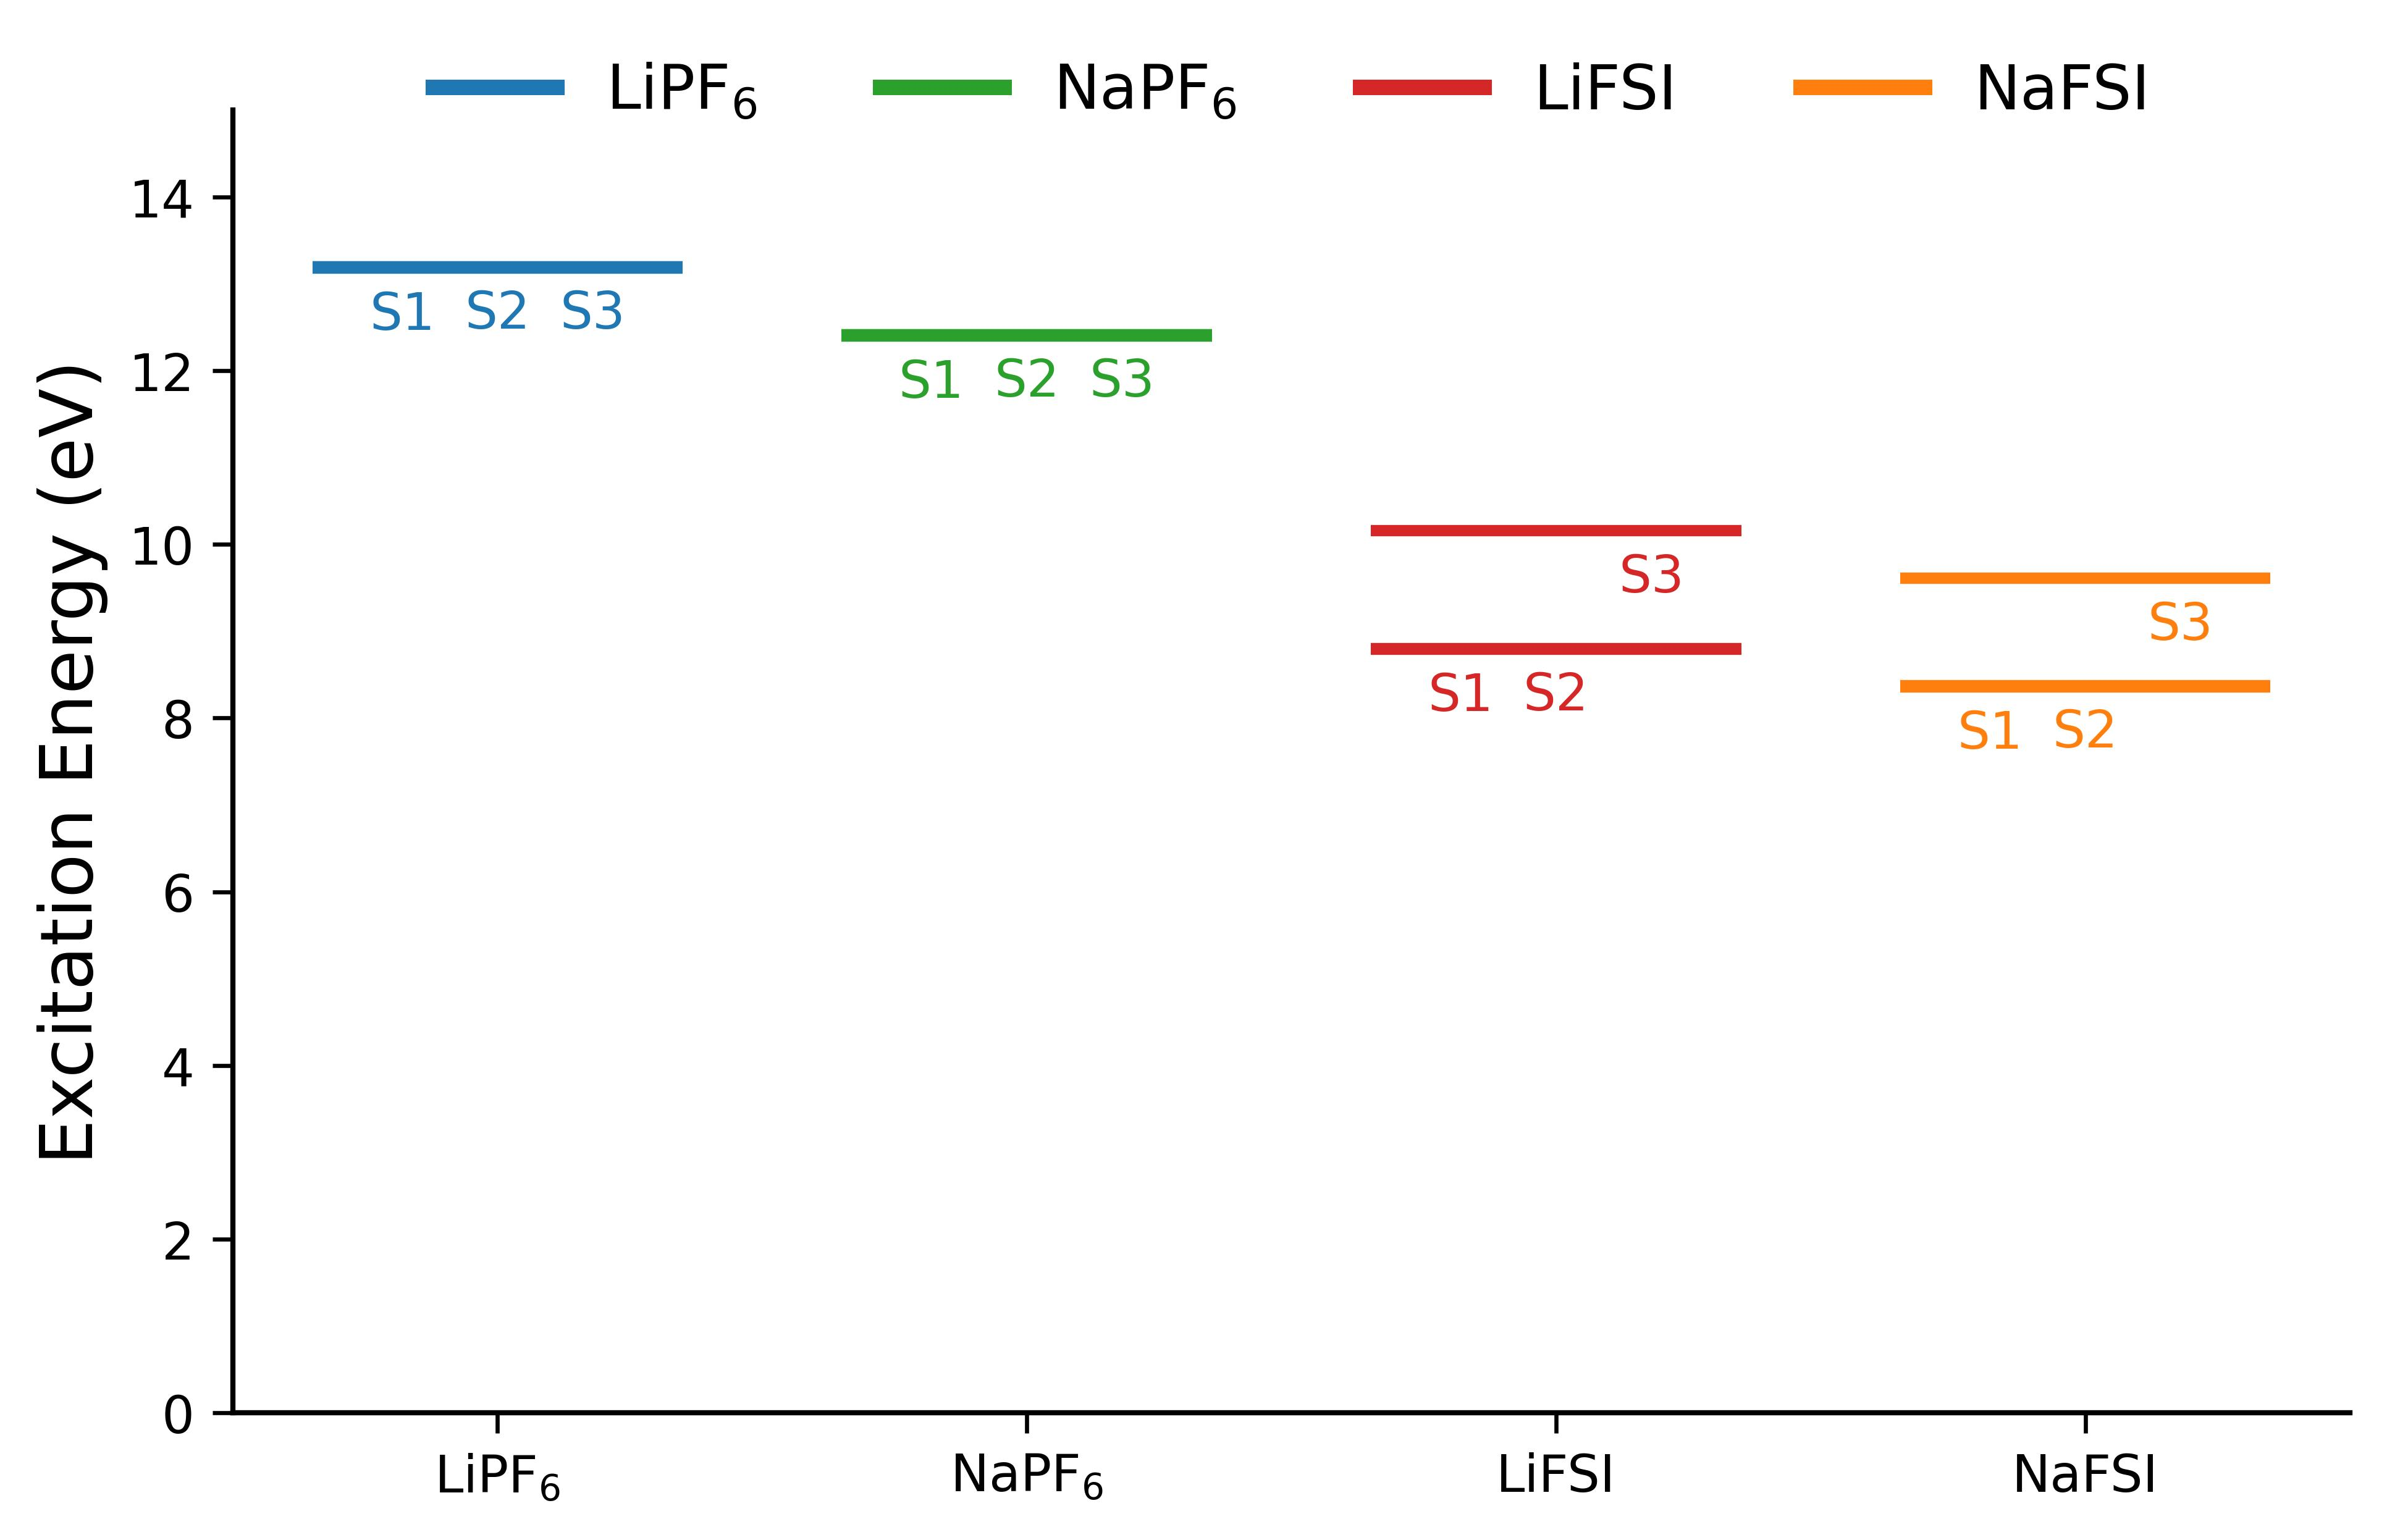
\includegraphics[width=12.5cm]{excitation_levels_electrolytes.jpg}
  \caption{Lowest singlet excitation energies (S$_1$--S$_3$) from VQE–qEOM for LiPF$_6$, NaPF$_6$, LiFSI, and NaFSI. 
  FSI salts show markedly lower S$_1$ (narrower gaps) than PF$_6$. 
  PF$_6$ exhibits a near–degenerate cluster at 12–13~eV, whereas FSI presents a near–degenerate pair (S$_1$, S$_2$) and a higher S$_3$ separated by $\sim$1.3~eV. 
  Deep–UV onsets (nm): LiPF$_6$~$\sim$94, NaPF$_6$~$\sim$100, LiFSI~$\sim$141, NaFSI~$\sim$148.}
  \label{fig:exciton_energy}
\end{figure}

The present analysis focuses on excitation energies; however, oscillator strengths are essential for assessing photostability and spectral intensity. 
Current qEOM implementations in Qiskit do not expose transition dipole moments directly. 
Future work will compute oscillator strengths from transition density matrices and analyze natural transition orbitals, enabling quantitative state assignments and brightness trends across the electrolyte series.

%\paragraph{Solvent effects and NISQ constraints.}
%All VQE–qEOM results reported here are obtained for isolated species or embedded cluster Hamiltonians that do not explicitly model the macroscopic solvent. 
%In the current NISQ regime, the qubit counts and circuit depths required for fully explicit solvation are prohibitive. 
%To nevertheless contextualize the spectra, we adopt hybrid quantum–classical strategies in which the quantum computer provides accurate gas-phase excitation energies for a compact active space, and the solvent shift is estimated classically.

%\emph{$\Delta$-solvation correction.}
%We estimate the solvated excitation by
%\[
%E^{\mathrm{QC}}_{\mathrm{solv}} \;\approx\; 
%E^{\mathrm{QC}}_{\mathrm{gas}} \;+\; 
%\big(E^{\mathrm{cl}}_{\mathrm{solv}} - E^{\mathrm{cl}}_{\mathrm{gas}}\big),
%\]
%where $E^{\mathrm{QC}}_{\mathrm{gas}}$ is the VQE–qEOM gas-phase value, and the bracket is a classical solvation shift obtained, e.g., from TDDFT with a continuum model (PCM/CPCM/SMD). 
%This assumes the dominant solvent effect is mean-field polarization, which is well captured by linear-response models.

%\emph{Static embedding potential.}
%Alternatively, a classical environment potential $v_{\mathrm{env}}(\mathbf r)$ (e.g., polarizable embedding, QM/MM point charges, or frozen-density embedding) can be folded into the one-electron operator,
%\[
%h_{pr}^{\mathrm{emb}} \;=\; h_{pr} 
%\;+\; \int \phi_p^*(\mathbf r)\, v_{\mathrm{env}}(\mathbf r)\, \phi_r(\mathbf %r)\,d\mathbf r,
%\]
%yielding an embedded second-quantized Hamiltonian for the VQE–qEOM step without increasing the qubit count.

%\emph{Minimal explicit clusters.}
%For specific first-shell effects (ion pairing, hydrogen bonds), we also consider small explicit solvent clusters and retain only the frontier orbitals of the chromophore in the active space, freezing the remainder. 
%This preserves NISQ tractability while capturing local, specific interactions.


%\section{Conclusion}
%In this work, we demonstrated that quantum algorithms can capture the essential electronic structure and photostability trends of technologically relevant electrolyte salts. By combining VQE with qEOM, supported by systematic active-space design and qubit reduction, we obtained chemically accurate ground- and excited-state energies for LiPF$_6$, NaPF$_6$, LiFSI, and NaFSI. Dissociation curve analysis and benchmarking against CASCI confirmed that VQE with reduced active spaces achieves sub-milliHartree accuracy, while SQD with extended qubit registers recovers near-exact results. Importantly, we identified three key insights: (i) PF$_6$ salts exhibit higher excitation thresholds and superior photostability compared to FSI salts; (ii) FSI salts, while optically more accessible, form deeper binding wells and stronger ionic interactions; and (iii) Na substitution consistently lowers excitation energies relative to Li, revealing systematic cation effects.

%Beyond establishing the accuracy of NISQ-era algorithms, our results highlight how quantum simulations can uncover chemically meaningful stability trends that are directly relevant to electrolyte degradation in lithium- and sodium-ion batteries. Looking ahead, extending this framework to solvated clusters, interfacial systems, and noisy quantum hardware will enable more realistic modeling of electrolyte environments. These developments mark a step toward using quantum computing not only as a validation tool but also as a predictive engine for designing stable, high-voltage electrolytes in next-generation energy storage technologies.


\section{Conclusion}
We have demonstrated that hybrid quantum algorithms can capture essential ground- and excited-state features of technologically relevant electrolyte salts. Using VQE for ground states and qEOM for vertical singlet excitations, supported by systematic active-space design, qubit reduction, and commuting-group measurements, we achieved close agreement with exact diagonalization within $\sim$10-qubit models. Extending to larger active spaces with sample-based quantum diagonalization (SQD) recovered near-exact (subspace-FCI) ground-state energies, providing a scalable benchmark.

Across LiPF$_6$, NaPF$_6$, LiFSI, and NaFSI, we identified robust spectral trends: (i) PF$_6$ salts possess higher first-excitation energies and a compact three-state manifold near 12--13~eV, whereas FSI salts exhibit lower onsets ($\sim$8--9~eV) with a (S$_1$,S$_2$) doublet and an S$_3$ $\sim$1.3~eV above; (ii) replacing Li$^+$ by Na$^+$ systematically narrows the optical gap by $\sim$0.4--0.8~eV within a given anion family; and (iii) dissociation profiles reflect stronger binding for FSI relative to PF$_6$ and for Li$^+$ relative to Na$^+$, consistent with ionic size and anion electronic structure. Taken together, these observations underscore distinct anion electronic environments and a reproducible cation dependence that are relevant to photostability and oxidative stability considerations.

The present study is limited to isolated species or embedded clusters compatible with NISQ resources; fully explicit solvation and interfacial effects remain out of reach for current hardware. In future work, we will integrate $\Delta$-solvation corrections (e.g., TDDFT/PCM or SMD), static or polarizable embedding into the one-electron operator, and transition-property evaluation (transition densities and natural transition orbitals) to obtain oscillator strengths and assign state characters. Hardware executions with calibrated error mitigation and expanded active spaces (including LUCJ/ADAPT ansätze and SKQD variants) will further test robustness. Overall, our results establish a reproducible quantum workflow for electrolyte screening and provide quantitative baselines to guide the rational design of next-generation battery materials.

Looking forward, the combination of active-space reduction, projector-based algorithms such as SQD, and error mitigation techniques will play a crucial role in enabling chemically meaningful quantum simulations on real hardware. As quantum devices continue to improve in coherence time and gate fidelity, incorporating systematic noise mitigation will allow the present framework to be extended beyond proof-of-principle studies toward predictive simulations of realistic electrolyte environments.


%%%%%%%%%%%%%%%%%%%%%%%%%%%%%%%%%%%%%%%%%%%%%%%%%%%%%%%%%%%%%%%%%%%%%
%% The "Acknowledgement" section can be given in all manuscript
%% classes.  This should be given within the "acknowledgement"
%% environment, which will make the correct section or running title.
%%%%%%%%%%%%%%%%%%%%%%%%%%%%%%%%%%%%%%%%%%%%%%%%%%%%%%%%%%%%%%%%%%%%%
\section*{Acknowledgements}

This work was supported by the Korea Institute of Science and Technology (Grant number 2E31851), GKP (Global Knowledge Platform, Grant number 2V6760) project of the Ministry of Science, ICT and Future Planning. The authors thank Shubhayu Das of RWTH Aachen for useful discussions.

\section*{Conflicts of interest}
The authors declare that they have no conflict of interest.
%%%%%%%%%%%%%%%%%%%%%%%%%%%%%%%%%%%%%%%%%%%%%%%%%%%%%%%%%%%%%%%%%%%%%
%% The same is true for Supporting Information, which should use the
%% suppinfo environment.
%%%%%%%%%%%%%%%%%%%%%%%%%%%%%%%%%%%%%%%%%%%%%%%%%%%%%%%%%%%%%%%%%%%%%
%\begin{suppinfo}

%\end{suppinfo}

\paragraph{Data availability.}
All geometries, active-space definitions, qubit Hamiltonians, and scripts to reproduce the VQE-qEOM and SQD results will be deposited in a public repository upon acceptance.

%%%%%%%%%%%%%%%%%%%%%%%%%%%%%%%%%%%%%%%%%%%%%%%%%%%%%%%%%%%%%%%%%%%%%
%% The appropriate \bibliography command should be placed here.
%% Notice that the class file automatically sets \bibliographystyle
%% and also names the section correctly.
%%%%%%%%%%%%%%%%%%%%%%%%%%%%%%%%%%%%%%%%%%%%%%%%%%%%%%%%%%%%%%%%%%%%%
\bibliography{ref}
\graphicalabstract{TOC_v2.jpg}
\end{document}


